\documentclass[11pt]{report}
\usepackage{graphicx}
\usepackage{subfig}
\usepackage{amsmath}
\usepackage{amssymb}
\usepackage{url}
\usepackage{bm}
\usepackage{setspace}
\usepackage[margin=2cm]{geometry}
\usepackage{epstopdf}
\usepackage{titlesec}
\usepackage{algorithm}
\usepackage{booktabs}
\usepackage[framed,numbered,autolinebreaks,useliterate]{mcode}
\usepackage[bookmarks,hidelinks,bookmarksnumbered=true,pdfstartview=FitH]{hyperref}

\titleformat{\chapter}
  {\Large\bfseries} % format
  {}                % label
  {0pt}             % sep
  {\huge}           % before-code

\newlength{\wideitemsep}
\setlength{\wideitemsep}{.5\itemsep}
\addtolength{\wideitemsep}{-7pt}
\let\olditem\item
\renewcommand{\item}{\setlength{\itemsep}{\wideitemsep}\olditem}

\DeclareMathOperator*{\argmin}{arg\,min}
\DeclareMathOperator*{\argmax}{arg\,max}
\renewcommand{\vec}[1]{\boldsymbol{\mathbf{#1}}}
\doublespacing

\begin{document}

\title{3rd Year Project Final Report \\ SleepAppnea}
\author{George Cochrane, Sachin Mylavarapu, Tuan Anh Le, Sophie Louth}

\maketitle

\begin{abstract}
The abstract text goes here.
\end{abstract}

\tableofcontents

\section{Introduction}
Lorem ipsum dolor sit amet, consectetur adipisicing elit, sed do eiusmod tempor incididunt ut labore et dolore magna aliqua. Ut enim ad minim veniam, quis nostrud exercitation ullamco laboris nisi ut aliquip ex ea commodo consequat. Duis aute irure dolor in reprehenderit in voluptate velit esse cillum dolore eu fugiat nulla pariatur. Excepteur sint occaecat cupidatat non proident, sunt in culpa qui officia deserunt mollit anim id est laborum.

\subsection{Subsection Heading Here}
Write your subsection text here. Add something. Add something else.
\chapter{The Condition}
\label{ch:medicalInfo}
Obstructive Sleep Apnoea (OSA), sometimes called hypersomnia sleep apnoea syndrome, occlusive sleep apnoea ~\cite{whitelaw1993characteristics}, sleep disordered breathing ~\cite{sleepdisorderedbreathing}, hyperventilation syndrome and Pickwickian Syndrome, however the latter three are discouraged because they are also used to describe other disorders, is a sleep disorder characterised by repetitive blockages in the upper airway during sleep, but with inspirational effort. These blockages can be apnoeas, full closure, or hypopnoeas, partial closure, both cause a restriction in airflow, which can lead to reduction in oxygen saturation and frequent arousal in order to re-establish airflow ~\cite{american2001international}.
The upper airways include the nasal cavity, oral cavity and pharynx, the area behind the tongue (see Figure \ref{fig:Sagittal-Face} ). The main part that becomes blocked is the pharynx, this is usually held open by the pharyngeal dilator muscles, although these relax during sleep in a healthy subject they are still able to maintain airflow, however in an OSA sufferer they provide insufficient force to prevent collapse ~\cite{fogel2004sleep}. Collapse only occurs during inspiration and is due to negative pharyngeal pressure. During rapid eye movement (REM) sleep there is further relaxation of the pharyngeal dilator muscle which can lead to longer apnoea and hypopnoea events. 
\begin{figure}[h]
\centering
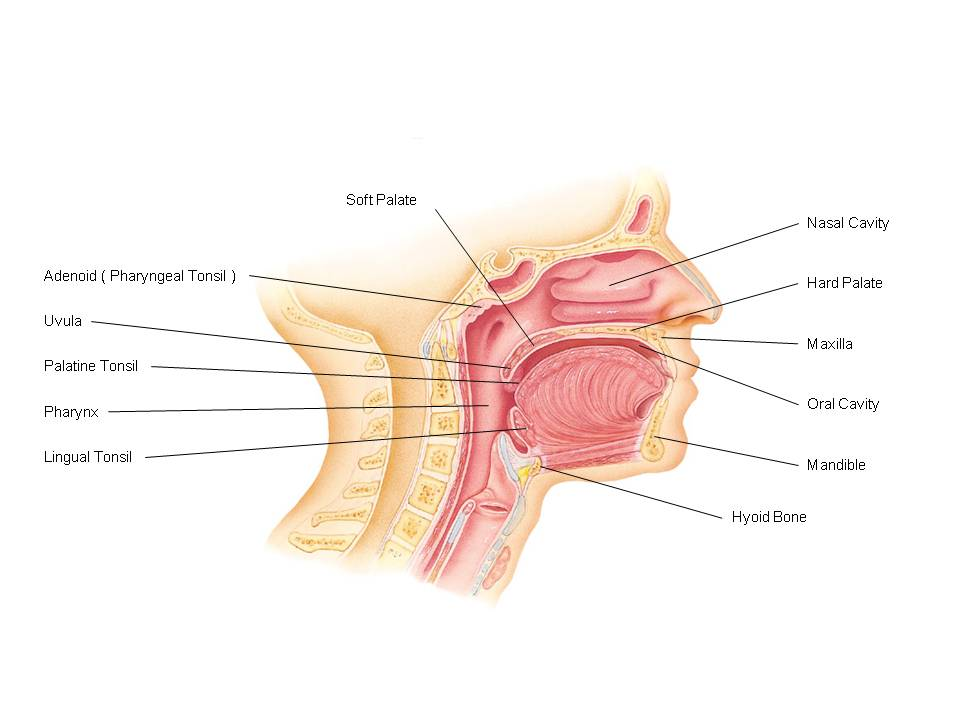
\includegraphics[width=0.9\textwidth]{drawings/Sagittal-Face}
\caption{Sagittal View of the Face to show Upper Airways ~\cite{sagittalface}}
\label{fig:Sagittal-Face}
\end{figure}
Many factors affect the likelihood a patient suffers with OSA, however one thing is consistent in almost all cases; the pharyngeal upper airway size is smaller than in normal patients and often more elliptical with the long axis directed anterior-posterior, rather than laterally as it is in non sufferers, which alters the pharyngeal dilator muscle orientation leading to a mechanical disadvantage, this can have a number of causes including fat deposits and facial bone structure ~\cite{leiter1996upper}. Overweight and obese patients often have fat deposits lateral to the pharynx, not always substantial but its positioning creates or reinforces elliptical shape, pharynx orientation and reduction in size. 
The main element of facial bone structure that influence upper airway size is the positioning and size of the maxilla and mandible (upper and lower jaw bones), these can influence the airway size in a couple of ways: micrognathia where the jaws are undersized, retrognathia ( or overbite) where the mandible is set back compared to the maxilla in both of these cases the tongue sits further back in the mouth, increasing tendency to block airflow. Lower positioning of the hyoid bone and Brachycephaly where the head is wider than it is tall can have a similar effect ~\cite{lowel1995cephalometric}.
Abnormal facial tissues can also have an effect, large tonsils and adenoids, elongated or enlarged uvula ( the dangly bit at the back of the mouth, see Figure \ref{fig: Anterior-View-Mouth}), macroglossia ( enlarged tongue), high arched or narrow hard palate, and reduced nasal patency ( cross sectional area) possibly caused by nasal abnormalities all have been shown to factor ~\cite{schwab1995upper}.
\begin{figure}[h]
\centering
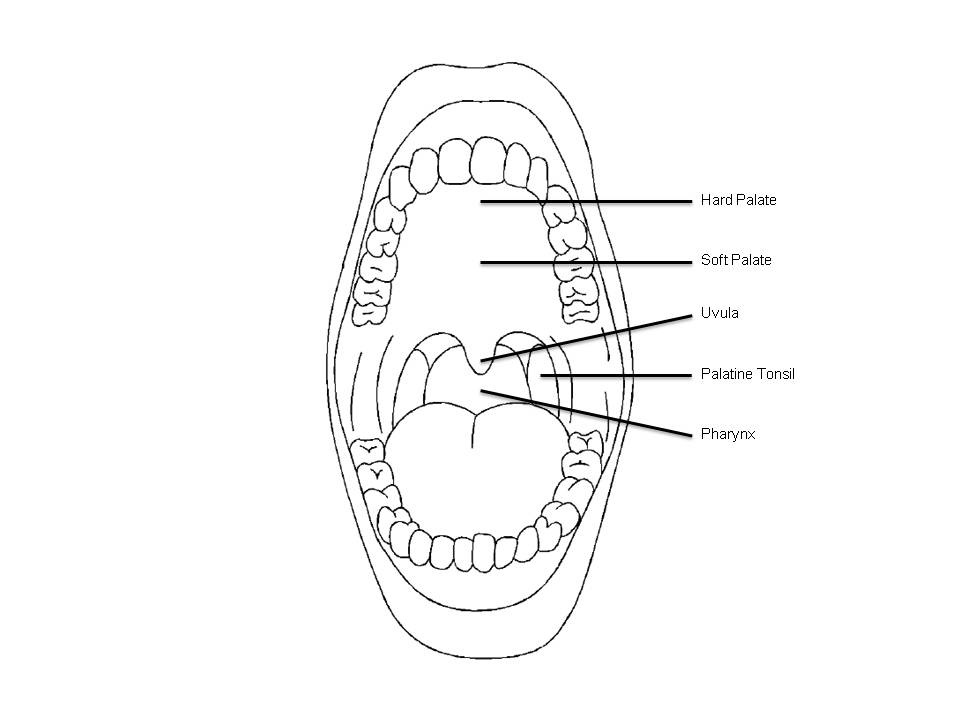
\includegraphics[width=0.6\textwidth]{drawings/Anterior-View-Mouth}
\caption{Anterior View of the Mouth to show Upper Airway Tissues~\cite{anteriormouth}}
\label{fig: Anterior-View-Mouth}
\end{figure}

Other factors include lying supine (on back) where gravity causes the tongue to fall into the airway. Some drugs including alcohol relax the pharyngeal dilator muscles more than just the effects of sleep, worsening OSA. Smoke irritates tissues including those in the upper airways, swelling them such that they cause a narrowing of the airway ~\cite{apneosotherfactors}.
 Severity of the Condition can be measured in two ways AHI and RDI. AHI or Apnoea Hypopnoea Index counts the average number of apnoeas and hypopnoeas per hour asleep. The severity is then classified as minimal if AHI <5, mild if 5<= AHI < 15, moderate 15<= AHI <30 and severe AHI>= 30. RDI or Respiratory Disturbance Index is similar but also includes respiratory-effort related arousals (RERAs) in the count ~\cite{AHI}. The same classifications are used as for AHI however this can be unhelpful given the RDI is likely to be higher than AHI for the same patient ~\cite{epstein2009clinical}.

\section{Rationale}
Lorem ipsum dolor sit amet, consectetur adipisicing elit, sed do eiusmod tempor incididunt ut labore et dolore magna aliqua. Ut enim ad minim veniam, quis nostrud exercitation ullamco laboris nisi ut aliquip ex ea commodo consequat. Duis aute irure dolor in reprehenderit in voluptate velit esse cillum dolore eu fugiat nulla pariatur. Excepteur sint occaecat cupidatat non proident, sunt in culpa qui officia deserunt mollit anim id est laborum.
\chapter{The app}
<<<<<<< HEAD
\section{Structure Of The App}
The app has been designed to have a very simple structure and layout so as to be immediately usable and comprehensible, even by those less technologically minded. Each activity branches from the main “welcome screen” activity, and upon completion of each activity, the user is the brought back to the “welcome screen” activity in order to select the next stage of the app to complete.
\begin{figure}[ht!]
		\centering
			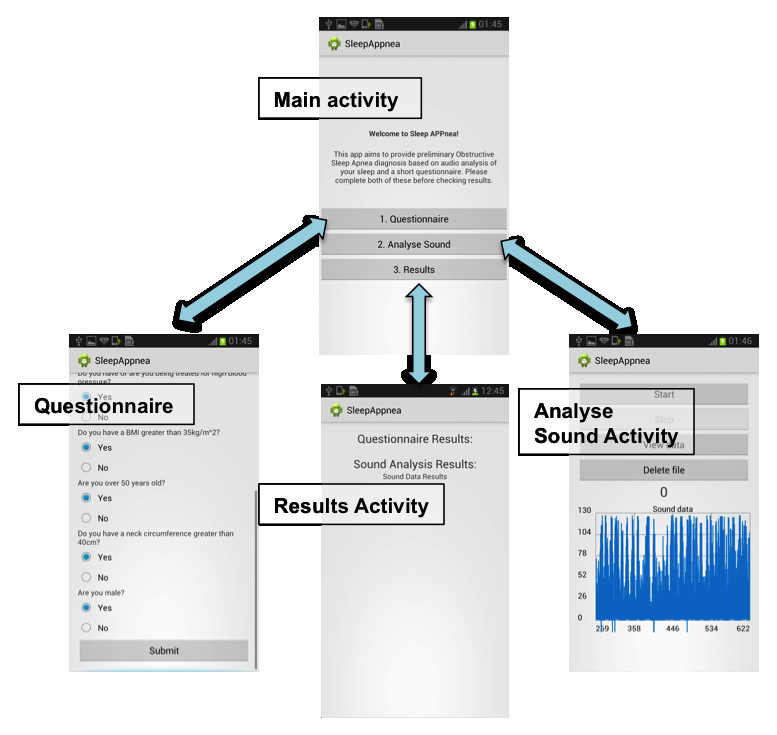
\includegraphics[width=.5\textwidth]{drawings/Structure-network.eps}
		\caption{Network view of the app's structure}
		\label{fig:appStructure}
	\end{figure}
\subsection{Home Activity}
The app loads into the home activity when it is first turned on. The user is welcomed to the app and given a brief explanation of how to use the app. Below this the user is presented with three buttons to launch the three other activities. 
\subsection{Questionnaire Activity}
The first task for the user to complete is the questionnaire, based on the eight STOPBANG criteria questions as detailed later in the ‘Design Process’ section of this report. Pressing the submit button then takes you back to the start page and simply stores the number of ‘yes’ answers the questionnaire received. This number is called during the processing of the overall results, noting that three or more ‘yes’ answers indicates a high risk of Obstructive Sleep Apnea. The default for all of the answers is ‘yes’ which should encourage the user to actively read/change each question (given that statistically the average person would have more ‘no’ answers). It also means that should the user bypass the questionnaire section or ignore the questions before hitting ‘submit’, the app will use the higher risk criteria and results will be more likely to suggest too high a probability of apnea than miss a positive diagnosis altogether. 
\subsection{Sound Analysis Activity}
This activity is indicated as the second task to complete, though it doesn’t require completion of the questionnaire before being executable itself. The user is presented with four simple buttons as seen below. Note the following button restrictions:
\begin{itemise}
\item ‘Stop’ cannot be pressed until the phone is recording audio.
\item ‘View Data’ and ‘Delete File’ do nothing until there is data stored (‘Nothing yet’ is displayed as an indicator’).
\item When ‘Start’ has been pressed, the ‘Stop’ button becomes the only usable button. This is done by checking whether the inbuilt Boolean variable ‘isRecording’ is true, and as such, the inverse becomes true again as soon as ‘Stop’ is pressed.
\end{itemise}
For this simple prototype of the app, recording is restricted to one file in any instance of the app running.
\\ The sound data is automatically stored to a file accessible only by the app and is later analyzed by the machine-learning algorithm and overall results algorithm. Clearly the delete button is only included for cases where recordings were accidentally created and as such, it uses a comprehensive ''Are you sure?'' alert upon pressing to avoid deletion of wanted files.
\\Progress bars are used whilst the sound is being saved and loaded which will reassure the user that the app is still running properly during these otherwise unresponsive stages of high CPU usage. 
\subsection{Results Activity}
In this activity, a simple algorithm is used to determine an overall probability that the user has obstructive sleep apnea, and brief medical advice is given accordingly. It combines the results of the questionnaire and the audio recording analysis to do this, and therefore if one of these two parts is not present, it will ask for the user to go back and complete it before full results are displayed. Again, all analysis and loading tasks that takes more than half a second or so utilize a progress bar for improved user interface.
\subsection{Navigation Around The App}
The buttons are intended to be as intuitive as possible for navigation of the app. Loading each extra activity can only be done from the home activity, and the activity is exited by pressing the hardware ''back'' button whilst on the home activity. Each extra activity exits back to the home activity upon pressing this ''back'' button too, though the Questionnaire has the same functionality added in to the ''Submit'' button which helps reassure the user that the button has indeed been pressed.

=======
\label{sec:app}
Lorem ipsum dolor sit amet, consectetur adipisicing elit, sed do eiusmod tempor incididunt ut labore et dolore magna aliqua. Ut enim ad minim veniam, quis nostrud exercitation ullamco laboris nisi ut aliquip ex ea commodo consequat. Duis aute irure dolor in reprehenderit in voluptate velit esse cillum dolore eu fugiat nulla pariatur. Excepteur sint occaecat cupidatat non proident, sunt in culpa qui officia deserunt mollit anim id est laborum.
>>>>>>> FETCH_HEAD

\chapter{Design Process}

\section{Diagnostic Methods}
There are four strategies used to approach diagnosis they are; the algorithmic method, pattern recognition method, hypothetico-deductive method; sometimes called differential diagnosis, and the exhaustive method. 
The algorithmic method uses flowcharts and algorithms to analyse data that are precise and reproducible for example vitamin B12 level in blood. One follows steps making decisions at preselected branch point based on the clinical data available. This relies on a flow chart for the illness and the illness to present in a relatively normal way. Abnormal presentation of an illness could easily lead to misdiagnosis. For example if an OSA sufferer is not overweight but instead has lateral peritonsular narrowing, they may well be missed by this method. 
The pattern recognition method, is best for conditions with distinct presentation, especially those which present regularly in the population. It is refered to as pattern recognition because the symptoms and signs displayed by the patient reawakens memories in the doctor of previous examples. It is an efficient method, especially useful when time critical diagnoses are needed. This does however risk jumping prematurely to a final hypothesis, although the consequences of this can be reduced by follow up in order to check instincts. 
The hypothetico-deductive method lends itself to primary care settings as it results in a differential diagnosis, a rank ordered list of hypotheses. Hypotheses are generated and rejected as more data are collected and questions asked until a working hypothesis is reached. This method is most often used as it reflects how most people deal with life, and is therefore the most natural. It can cause errors if a doctor has been exposed to a certain diagnosis recently, they may choose to ignore signs that what they are looking at is in fact not that. For example if a doctor has diagnosed and number of patients with OSA recently ( or read a paper about it) they may diagnose a patient who expresses day time sleepiness and witnessed apneas with OSA when in fact the previous traumatic head injury would be an indicator for Central Sleep Apnea, in this case a polysomnogram would be needed to see whether the patient was actually attempting respiration during apneas. Another error situation can be caused by the doctor failing to think about the probability of a diagnosis being correct. for example, if a patient presents with witnessed choking during sleep as the primary symptom rather than daytime sleepiness or witnessed apneas the doctor may diagnose Sleep Choking Syndrome however this has a much lower prevalence than OSA, rare compared to about 2-4% for OSA.
The exhaustive method works on the premise of having all the information, all data collected, all questions asked. Completeness of data is important for hospitalised patients but acquiring it is too time consuming and expensive for most cases. Useful for unusual illness when other methods have failed or for unusual expressions of illnesses. 
The hypothetico-deductive method will be useful in order to establish what symptoms and signs can be used to differentiate OSA from other disorders. However the app itself will need to rely on pattern recognition because ruling out all options will be impossible as a doctor won’t be administering the app. It was also be unnecessary to use an exhaustive method as the app is only designed to pick up OSA not all sleep disorders or reasons for daytime tiredness. 

\section{Signs and Symptoms – non invasive methods}
Table X shows all the known signs and symptoms of OSA along with detectable presentation. From there Table X+1 shows these presentations and the different sensors for measuring them, as well as whether those sensors are invasive or not. The non-invasive sensors shall be the focus of the following work. The presenting symptom for OSA is daytime sleepiness, with reports of snoring and witnessed apneas from the patient’s bed partner. So focussing on other conditions with these symptoms is a start to finding a unique combination of symptoms for OSA that can be tested non-invasively by an app. 
Table X+2 looks at four key symptoms of OSA which the majority of patients display ( and can be detected non-invasively). Disorders which also display one or more of these symptoms are then listed along with their differentiator from OSA. From the table it is clear most of these conditions can be ruled out by diagnosis focussing on daytime sleepiness, snoring, and an apnea awakening/choking combination. 
Ascertaining these would eliminate all but central sleep apnea and altitude insomnia however both of these would be picked up a significant proportion of the time by a questionnaire because the sufferers would only fit the risk cases for OSA in a small percentage of cases. Especially for altitude insomnia as those with a BMI over 35kgm-2 are unlikely to be climbing over 4000m in height for extended periods ( i.e. climbing mountains rather than flying).
Those suffering from central sleep apnea are likely to reflect population distribution for BMI as weight is not a cause or exacerbating factor. I.e. about 25% of central sleep apnea patients are obese ( BMI >30) compared to 70% of OSA sufferers.
Methods are then needed to detect daytime sleepiness, loud snoring and apnea arousal ( choking) combinations. Sensors to look at are; video, accelerometry, audio and questionnaires. Idea and their merits and weaknesses will be discussed next.

\subsection{Video}
The aim is to pick up on apneas via cessation of breathing and arousal via significant body movement. Snoring would not be possible to detect although some other attributes that hint at OSA may be detectable e.g. lying in the supine position ( on back). Video could also be used to detect sleep and activity, e.g. sleep cycle transitions and limb movements. 
Merits include, smartphone already have cameras so an external camera wouldn’t be needed, although the cameras may struggle with the low light level in the sleeping space, and changing the light level in order to accommodate the camera could have a knock on effect on the quality or type of sleep. 
Weaknesses include, positioning of the camera will be important and this is hard when all rooms are different and smartphones don’t naturally stand up by themselves. Manual analysis of the video has been used until recently so there isn’t a great deal of statistical data on how well computer algorithms can detect OSA. Video produces large data files that cannot be sensibly stored on a phone. Video has formed part of the polysomnogram in some areas for a long time as an aide to observation and only recently investigated as an independent method of diagnosis using automated analysis. As a consequence lots of video data does exist however it is highly regulated due to patient confidentiality. 

\subsection{Accelerometry}
This has the potential to be able to detect body position and sleep wake segmentation which could give a pretty good indicator of apnea arousal events, however mechanism for detecting snoring.
This has not been part of the polysomnogram although it has started to be investigated as a mechanism for detecting OSA. There is very little data available which makes a retrospective study a challenge, especially as there is no data conbined with polysomnogram data for verification. Positioning of the phone in order to get the best results without damaging the phone would require some investigation. Non standardised arrangements of mattress and bed clothes may cause issues. 

\subsection{Audio}
The most obvious way to detect audio signals from the patient is via the phone’s in built microphone although external microphones should also be investigated. It ought to be possible to detect apnea arousal events and snoring. 
Lots of work has been done on audio analysis of speech so there are lots of ideas out there to work from. Many polysomnograms include a sound recording for reference so there is a lot of data available and in the most part it is anonymised so there isn’t a risk to patient confidentiality. In some cases it has been labelled so it can be used easily for a retrospective study such as this one. There are also regulations which can act as a guidline. 

\subsection{Questionnaire}
A questionnaire is pretty much the only way to assess daytime sleepiness, it can also be used to acquire about other symptoms and co-morbidities. If a prexisting questionnaire is used then there will be data on its effectiveness and usability and statistics it has produced. Questions for part of the diagnostic pathway so it takes some of the work away from the doctor. Some studies show patients are more truthful with anonymous questionnaires than with their doctor, more on that to follow.

\subsection{Conclusion}
Given that audio analysis and questionnaires should be sufficient to diagnose OSA and rule out other similar disorders, these will be investigated further with the other methods discarded unless significant issues are encountered with audio and questionnaire analysis.

\newpage
\section{Questionnaire selection (Sophie)}
\label{sec:questionnaire-sophie}
The key point that needs to be established via the questionnaire is whether the patient suffers from daytime sleepiness. However knowing about the patient’s weight can be useful to eliminate central sleep apnoea, and other questions about symptoms can be useful to reinforce diagnosis. 

\subsection{New vs. Pre-existing Questionnaire}
 There is a key decision between two options at this stage: to create a new questionnaire from scratch or to use a pre-existing questionnaire. A new questionnaire gives much more freedom as to what questions to ask in order to target particular symptoms and eliminate other disorders. It also allows for unique methods of analysis e.g. weighted questions rather than a simple threshold based on number of questions answered. Rigorous market research can be used to design the wording of the questions to maximise truthfulness and ease of interpretation, as well as number of questions and mechanism of answering. However this would be time consuming and an expert in question production is potentially needed. Data from patients would need to be collected via the questionnaire and other means in order to test its effectiveness, i.e. it could not be used as a retrospective study.

Using a pre-existing questionnaire allows for quicker set up time as there will either be data available in order to validate the questionnaire or it will have already been validated. Some questionnaires are within the doctor’s guideline so time can be saved during consultation if they are already performed. Named questionnaires are often recognised by doctors which saves them time checking the questions.

Given the time constraints and the access to data and skills, further investigation will look at pre-existing questionnaires. 
\subsection{Using app based questionnaires to increase patient truthfulness}
One of the benefits of performing questionnaires on the app rather than waiting for patients to attend an appointment is saving doctors time. However there is another benefit in the form of potentially increased truthfulness. 

Castelo-Branco et al found that patients tended to lie in order to look good, in the context of sexuality, when those involved had a strong interest in not giving a disappointing impression ~\cite{castelo2010patients}. Rogers looked at doctors’ trust in patients which is an indicator of suspected lying ~\cite{rogers2002there}. Ulterior motives were thought to have a significant influence on patients’ truthfulness. In the case of OSA there is a risk of patients playing down daytime sleepiness in order to avoid diagnosis if they wish to avoid having to contact the DVLA and their car insurance company and risk losing their license or insurance due to misunderstanding. There is also a case that patients may try and get a diagnosis in order to receive disability related financial support. However tricking a sleep test into thinking you have OSA would be challenging. 

\subsection{Questionnaires}
There are a number of questionnaires that have been used to assess diagnosis of OSA: some rely on a doctor to measure physical features, others use characteristic clinical features, others use patients’ interpretations of their symptoms, and the rest use combinations of the above. 

\begin{itemize}
\item Chung et al – STOP Questionnaire \\
Four questions on snoring, daytime sleepiness, witnessed apnoeas and blood pressure ~\cite{chung2008stop}.
\item Chung et al –STOPbang Questionnaire \\
This is an extension of the STOP questionnaire that adds four additional questions on BMI, age, neck circumference and gender. A threshold of 3 out of 8 is generally used to indicate OSA ~\cite{chung2012high}.
\item Chung et al – ASA \\
Three categories are used to ask questions: physical characteristics, observed sleep disturbances and tiredness. It uses falling into two or more of these categories as an indicator of OSA ~\cite{chung2008validation}.
\item Dixon et al \\
Looked at witnessed apnoeas, neck circumference and BMI. Study rather than a questionnaire ~\cite{dixon2003predicting}.
\item Flemons’ et al – Flemons’ screening tool \\
This is a 36 question screening tool for OSA that uses a differential method for diagnosis, asking questions about depression and chronic diseases as well as the more common questions on tiredness, snoring and driving behaviour. Uses a weighted score called SACS with a threshold to indicate OSA ~\cite{flemons1994likelihood}.
\item Kirby et al – Artificial Neural Nets \\
Uses 23 clinical variables including patient’s history, physical examination and patient reported sleepiness and smoking ~\cite{kirby1999neural}.
\item Kushida et al – Kushida Index \\
Complicated morphometric model, including BMI, neck circumference, palatal height and oral cavity measurements amongst others. Suffers from being too complicated to be administered accurately and being time consuming ~\cite{kushida1997predictive}.
\item Maislin et al \\
Model incorporates snoring, gasping at night, witnessed apnoeas, age, gender and BMI. Multiple logistic regressions were used to generate a multivariable apnoea risk register when compared to RDIs from polysomnographs. ROCs were used to test predictive ability ~\cite{dinges1995survey}.
\item Netzer et al – Berlin Questionnaire \\
Uses ten questions about snoring, witnessed apnoeas, daytime sleepiness, sleeping while driving, high blood pressure and BMI. Analysis is via simple scoring ~\cite{netzer1999using}.
\item Rosenthal and Dolan – Epworth Sleepiness Scale \\
A questionnaire using eight questions to assess sleepiness in different situations. Recommended by NHS guidelines ~\cite{rosenthal2008epworth}.
\item Tsai et al - Upper Airway Physical Examination Protocol \\
Looked at six parameters: three clinical symptoms; snoring, witnessed apnoeas and hypertension; and three measurable signs; cricomental space, pharyngeal grade and overbite (info on these to follow) ~\cite{tsai2003decision}.
\item Viner et al\\ 
Model incorporates snoring, BMI, age and gender. Used stepwise linear logistic regression ~\cite{viner1991history}.
\end{itemize}

\subsection{Narrowing Down the Studies}
There are too many questionnaires to look at all in detail. However given they are not all suitable for use in a mobile app they can be reduced in number and those that are more appropriate assessed. The Kushida Index and ASA questionnaire are complicated, which goes against the design specification, so can be discounted. Table \ref{table:questionnaire} shows the statistics the studies found for each questionnaire. A high negative predictive value is needed so the focus of more work will be on; Artificial Neural Net, UAPP and the STOPbang questionnaire. Epworth Sleepiness Scale will also be investigated for use in the app because it is part of the diagnostic pathway as laid out by the NHS.

\begin{table}[h]
\centering
\begin{tabular}{l l c c c c c c}
\toprule
Study&Test&n&Sens&Spec&Likelihood Ratio&NPV&PPV\\ \midrule
Chung et al&STOP&177&74&53&1.57&76&51\\ 
Chung et al&STOPbang&177&93&43&1.63&90&52\\ 
Chung et al&ASA&177&79&37&1.25&73&45\\ 
Dixon et al&&99&96&71&3.31&&\\ 
Flemons' et al&Flemons' screening tool&180&&&5.17&&81\\ 
Kirby et al&Artificial neural net&405&99&80&4.95&98&88\\ 
Kushida et al&Kushida index&300&98&100&large&88.5&100\\ 
Maislin et al&&427&60&&&&\\ 
Netzer et al&Berlin questionnaire&744&86&77&3.74&&89\\ 
Rosenthal&Epworth sleepiness scale&268&76&31&&&\\ 
Tsai et al&UAPP&75&40&96&10&100&95\\ 
Viner et al&&410&94&28&1.31&&\\ \bottomrule
\end{tabular}
\caption{Questionnaire Statistics based on an AHI \textgreater 15 threshold. n, number in the study, Sens, sensitivity (\%); Spec, specificity (\%),NPV, negative predictive value (\%), PPV, positive predictive value (\%).}
\label{table:questionnaire}
\end{table}
\subsection{Artificial Neural Net}
The 23 clinical variables which form the parameters for the neural network are shown in Table \ref{table:neural}. The patient would be aware of the demographics and social history information. However night time symptoms and bed partner observations would be more challenging and impossible for the patient to know about themselves in some cases. As regards past medical history, anthropometrics and the physical examination, in most cases the patient would not be able to self administer the questionnaire, negating its use.
\begin{table}[h]
\centering
\begin{tabular}{l l}
\toprule
Variables&Characteristics\\ \midrule
Demographics&Age, gender\\ 
Night time symptoms&Frequent awakening, experienced choking\\ 
Bed partner observations&Witnessed apnoeas, observed choking\\ 
Daytime symptoms&Reported excessive daytime sleepiness, Epworth sleepiness scale\\ 
Past medical history&Hypertension\\ 
Social history&Alcohol consumption, smoking in pack-yr\\ 
Anthropometrics&Height, weight, BMI, systolic BP ≥ 140, diastolic BP ≥ 90\\ 
Physical examination&Tonsillar enlargement, soft palate enlargement, crowding of the oral pharynx\\ 
Clinical score&Sum of the clinical scores for the binary categorical values (maximum score = 12)\\ \bottomrule
\end{tabular}
\caption{Patient Demographics and Clinical Features Used in the Neural Network of Prediction of OSA}
\label{table:neural}
\end{table} 

\subsection{Upper Airway Physical Examination Protocol}
This is only based on three features as shown in the flowchart(Figure \ref{fig:flowchart}: cricomental space, pharyngeal grade and overbite. All of these are physiological features hence their success at diagnosing OSA. However because they are physiological features there is a chance the patient would make significant errors while undertaking the readings. Cricomental space is the perpendicular distance from the cricomental line (which joins the cricoids cartilage in the neck to the chin) to the skin of the neck (see Figure \ref{fig:cricomental}), this is really hard to measure on yourself. Pharyngeal Grade measures how much the tonsils and other tissues at the back of the throat obscure the airway(see Figure \ref{fig:pharyngeal}). This is generally graded by eye and therefore might be possible for a patient to self assess. Overbite is where the top teeth are significantly in front of the bottom teeth; this is something a patient is generally aware of. When Tsai et al studied the UAPP as a diagnostic tool they had two different specialists assess the patients which reduces confidence in patients own ability to undertake such assessments. 

\begin{figure}[h]
\centering 
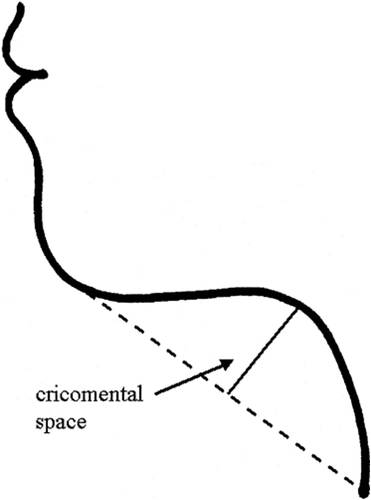
\includegraphics[width=0.2\textwidth]{drawings/cricomental}
\caption{Assessment of the cricomental space. Use a thin ruler to connect the cricoid cartilage to the inner mentum. The cricomental line is bisected, and the perpendicular distance to the skin of the neck is measured ~\cite{tsai2003decision}.}
\label{fig:cricomental}
\end{figure}
\begin{figure}[h]
\centering 
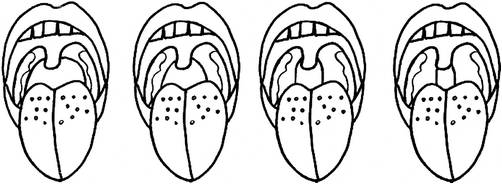
\includegraphics[width=0.4\textwidth]{drawings/pharyngeal}
\caption{Pharyngeal grading system. Class I = palatopharyngeal arch intersects at the edge of the tongue. Class II = palatopharyngeal arch intersects at 25\% or more of the tongue diameter. Class III = palatopharyngeal arch intersects at 50\% or more of the tongue diameter. Class IV = palatopharyngeal arch intersects at 75\% or more of the tongue diameter ~\cite{tsai2003decision}.}
\label{fig:pharyngeal}
\end{figure}
\begin{figure}[h]
\centering 
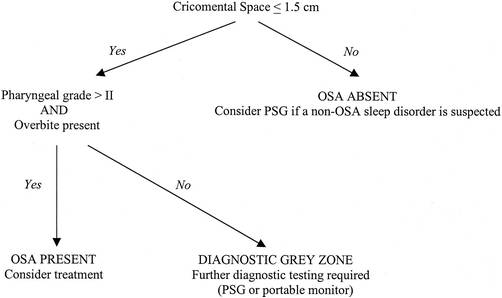
\includegraphics[width=0.5\textwidth]{drawings/flowchart}
\caption{A decision rule for diagnostic testing in OSA ~\cite{tsai2003decision}.}
\label{fig:flowchart}
\end{figure}


\subsection{STOPbang Questionnaire}
This questionnaire is based on eight questions to do with patients self reported symptoms. Each is answered with yes or no and the score is just a summation of the yes answers. Chung et al found that it was particularly good at distinguishing between severity of OSA, however as a simple diagnostic tool to find everyone who suffers it is relatively effective when used with a cut off of scoring 3 or above, with a probability of 93\% for detecting moderate OSA sufferers with AHI$\geq$15.

1. Snoring: Do you snore loudly (loud enough to be heard through closed doors)?
2. Tired: Do you often feel tired, fatigued, or sleepy during daytime?
3. Observed: Has anyone observed you stop breathing during your sleep?
4. Blood pressure: Do you have or are you being treated for high blood pressure?
5. BMI: BMI more than $35 \text{ kg} \text{m}^{−2}$?
6. Age: Age over 50 yr old?
7. Neck circumference: Neck circumference $>$ 40 cm?
8. Gender: Male?

\subsection{Epworth Sleepiness Scale}
This is a tool for establishing how much the patient feels they suffer from daytime sleepiness. The patient is asked to say how likely they are to doze in eight situations with 0 being they would never doze, through slight and moderate to high chance of dozing given a 3. A cut off value of 8 has been proposed by Rosenthal and Dolan which gives a sensitivity of 76\% for an AHI $\geq$5. 

Sitting and reading\\
Watching TV\\
Sitting, inactive in a public place (e.g. a theater or a meeting)\\
As a passenger in a car for an hour without a break\\
Lying down to rest in the afternoon when circumstances permit\\
Sitting and talking to someone\\
Sitting quietly after lunch without alcohol\\
In a car, while stopped for a few minutes in traffic

\subsection{Conclusion}
The STOPbang questionnaire and Epworth Sleepiness Scale are the only tests that a patient could reliably self administer, due to their shortness of length, ease to understand by a patient and ease to interpret by an algorithm. Both will be included in the app.


\newpage
\section{Signal Analysis -- simple method}

\newpage
\section{Machine Learning -- Theory}

\paragraph{}
	Machine learning, a branch of artificial intelligence, concerns the construction and study of systems that can learn from data \cite{wiki:machineLearning}. The supervised classification problem in machine learning concerns finding the unknown target function that classifies certain input data into classes based on some set of training examples containing labelled input data.
	
\paragraph{}
	In our case, given a sampled sound signal of a sleeper, we want to identify apnoea periods. In particular, we represent our input (sampled sound signal) as $\left\{s_1, s_2, \dotsc, s_T \right\} \equiv \left\{ s_i \right\}_{i = 1}^{T}$, and we want to output the classifiers for every $K$ samples, $\left\{ y_i \right\}_{i = 1}^{T/K}$, where the classifier $y_i \in \left\{0, 1\right\}$ corresponds to samples $\left\{ s_j \right\}_{j = \left(i - 1\right)K + 1}^{iK}$ of the signal. We assume that $T$ is divisible by $K$, however if this is not the case, we discard an appropriate number of signal samples to make it so.
	
\paragraph{}
	We have researched three models for our problem which we will discuss in this section. Firstly, we will discuss Support Vector Machines which are one of the most widely used algorithms in Machine Learning today, then we will discuss the State-Space and Hidden Markov Models, which turn out to be more well-suited to our problem due to their temporal nature. Moreover, we discuss techniques to condition our data before using them as input data for our learning models.
	
\subsubsection{Support Vector Machines}
\subsubsection*{State-Space Models}

\paragraph{}
	Here, we present the State-Space Models (SSMs) (also known as Linear Dynamical Systems) based on Kevin Murphy's book \cite[Chapter 18]{mlBook}. SSMs allow us to model systems that are dynamic. Unlike the SVMs, SSMs will model dependencies of the current state on the previous ones.
\subsection{Hidden Markov Models}

\paragraph{}
	Here, we present the Hidden Markov Models (HMMs), one of the most popular statistical models in machine learning with applications in many fields including but not limited to Cryptanalysis, Speech recognition and Bioinformatics \cite{wiki:HMM}. The material presented here is based on \cite{rabiner1989tutorial}, \cite{ramage07} and \cite{mlBook}. We will first present HMMs with discrete observations, then we extend this to include models with continuous observations.
	
\subsubsection{Discrete observations}
\paragraph{}
	Similarly to SSMs, we have two sets of random variables. Observed variables $\vec Y = \{ y_t \}_{t = 1}^T$ which are drawn from the observation alphabet $V = \{v_1, \dotsc, v_M\}$, and hidden states $\vec X = \{ x_t \}_{t = 1}^T$ which are drawn from the hidden state alphabet $S = \{ s_1, \dotsc, s_N \}$. The probabilistic graphical model of the HMM is identical to the one in Figure \ref{fig:pgm}. The hidden states obey Markov assumptions, i.e. $P( x_t | x_{t - 1}, \dotsc, x_1) = P(x_t | x_{t - 1}) = \text{const.}, t = 2, \dotsc, T$. Moreover, the observed variables are only dependent on the corresponding hidden state, i.e. $P( y_t | x_t, \dotsc, x_1, y_{t - 1}, \dotsc, y_1) = P(y_t | x_t), t = 1, \dotsc, T$.
	
\paragraph{}
	We parameterise a HMM using the transition matrix $\vec A$, emission matrix $\vec B$, and the initial state distribution $\vec \pi$. The transition matrix $\vec A \in \mathbb{R}^{N \times N}$ describes the transitions between hidden states, $A_{ij} = P(x_{t + 1} = s_j | x_t = s_i)$. The emission matrix $\vec B \in \mathbb{R}^{N \times M}$ describes the probability of an observation conditioned on a hidden state, $B_{jk} = B_{j}(v_k) = P(y_t = v_k | x_t = s_j)$. The initial state distribution $\vec \pi \in [0, 1]^N$ simply describes the initial probabilities of the hidden state, $\pi_i = P(x_1 = s_i)$. The model is fully described if we know these parameters, which we group into what is called a parameter set of the model, $\lambda = (\vec A, \vec B, \vec \pi)$.
	
\paragraph{}
	The three main questions of a HMM are
	\begin{enumerate}
		\item Find the probability of observations given the model, $P\left(\vec Y; \lambda\right)$.
		\item Find the most likely series of hidden states $\vec X$ to have generated the observations $\vec Y$, $\vec X^\ast = \argmax_{\vec X} P\left(\vec Y | \vec X; \lambda\right)$.
		\item Find the parameters $\lambda$ to maximise $P\left(\vec Y; \lambda\right)$.
	\end{enumerate}
We will discuss algorithmic solution to these three problems in turn.

\paragraph{Solution to the first problem.} To find the probability of an observed sequence, we use the dynamic programming algorithm, called the \textsc{Forward procedure} (outlined in Algorithm \ref{alg:forward}) which calculates the forward variable $\alpha_t (i) = P(\vec Y, x_t = s_i; \lambda)$.
\begin{algorithm}
	\caption{\textsc{Forward Procedure} for computing $\alpha_t(i)$.}
	\label{alg:forward}
	\begin{enumerate}
		\item
			\textbf{Initialisation.}
			$$\alpha_1(i) = \pi_i B_i(y_1), 1 \leq i \leq N$$
		\item
			\textbf{Induction.}
			\begin{equation*}
				\alpha_{t + 1}(j) = \left[ \sum_{i = 1}^N \alpha_t(i) A_{ij} \right] B_j (y_{t + 1}), 
				\begin{array}{lr}
					1 \leq t \leq T - 1\\
					1 \leq j \leq N
				\end{array}
			\end{equation*}
			
		\item
			\textbf{Termination.} (solution to the first problem)
			$$P\left(\vec Y; \lambda\right) = \sum_{i = 1}^N \alpha_T(i)$$
	\end{enumerate}
\end{algorithm}
As we can see, the algorithm has a time complexity of $O(TN)$.

\paragraph{Solution to the second problem.} 
	To solve the problem of finding the most likely sequence of hidden states, we use the \textsc{Viterbi Algorithm} proposed by Andrew Viterbi in 1967. The most likely sequence of hidden states is also called the Viterbi path. Firstly, we define the quantity $\delta_t(i)$, which stores the highest probability along a single path ending at the state $x_t = s_i$:
	\begin{equation}
		\delta_t(i) = \max_{x_1, \dotsc, x_{t - 1}} P\left( x_1, \dotsc, x_{t - 1}, x_t = s_i, y_1, \dotsc, y_t; \lambda \right)
	\end{equation}
By induction, we have
	\begin{equation}
		\delta_{t + 1}(j) = \left[ \max_i \delta_t(i) A_{ij} \right] B_j(y_{t + 1})
	\end{equation}
We also keep track of the index of the hidden state that maximises this quantity in
	\begin{equation}
		\psi_{t + 1}(j) = \argmax_i \delta_t(i) A_{ij}
	\end{equation}
Having defined these quantities, we present the \textsc{Viterbi Algorithm} in Algorithm \ref{alg:viterbi}.
\begin{algorithm}
	\caption{\textsc{Viterbi Algorithm} for computing the most likely sequence of hidden states.}
	\label{alg:viterbi}
	\begin{enumerate}
		\item
			\textbf{Initialisation.}
			\begin{align*}
				\delta_1(i) & = \pi_i B_i(y_1), & 1 \leq i \leq N \\
				\psi_1(i) & = 0, & 1 \leq i \leq N
			\end{align*}
		\item
			\textbf{Recursion.}
			\begin{align*}
				\delta_t(j) & = \max_{1 \leq i \leq N} \left[ \delta_{t - 1}(i) A_{ij} \right] B_j(y_t), &
				\begin{array}{lr}
					2 \leq t \leq T\\
					1 \leq j \leq N
				\end{array}\\
				\psi_t(j) & = \argmax_{1 \leq i \leq N} \left[ \delta_{t - 1}(i) A_{ij} \right], &
				\begin{array}{lr}
					2 \leq t \leq T\\
					1 \leq j \leq N
				\end{array}
			\end{align*}
		\item
			\textbf{Termination.}
			\begin{align*}
				P^\ast & = \max_{1 \leq i \leq N} \delta_T(i)\\
				x_T^\ast & = \argmax_{1 \leq i \leq N} \delta_T(i)
			\end{align*}
		\item
			\textbf{Path backtracking.}
			\begin{equation*}
				x_t^\ast = \psi_{t + 1}\left(x_{t + 1}^\ast \right),  T - 1 \geq t \geq 1
			\end{equation*}
		\item
			\textbf{Return $\left\{x_t^\ast \right\}_1^T$.}
	\end{enumerate}
\end{algorithm}
As we can see, the algorithm has a time complexity of $O(TN^2)$.

\paragraph{Solution to the third problem.}
	To learn the parameters of the model, $\lambda = \left( \vec A, \vec B, \vec \pi \right)$, we use the \textsc{Forward-Backward Algorithm} by Baum-Welch. We will need to introduce few quantities. Firstly, we introduce the backward variable $\beta_t(i) = P\left( y_{t + 1}, \dotsc, y_T | x_t = s_i; \lambda \right)$ which can be computed using a dynamic programming algorithm in Algorithm \ref{alg:backward}.
	\begin{algorithm}
		\caption{\textsc{Backward Algorithm} for computing $\beta_t(i)$.}
		\label{alg:backward}
		\begin{enumerate}
			\item
				\textbf{Initialisation.}
				$$\beta_T(i) = 1, 1 \leq i \leq N$$
			\item
				\textbf{Induction.}
				\begin{equation*}
					\beta_t(i) = \sum_{j = 1}^N A_{ij} B_j(y_{t + 1}) \beta_{t + 1}(j), 
					\begin{array}{lr}
						T - 1 \leq t \leq 1\\
						1 \leq j \leq N
					\end{array}
				\end{equation*}
		\end{enumerate}
	\end{algorithm}
We also define the variable $\gamma_t(i) = P\left( x_t = s_i | \vec Y; \lambda \right)$ which can be expressed as
	\begin{align}
		\gamma_t(i) 	& = P\left( x_t = s_i | \vec Y; \lambda \right) \nonumber\\
				& = \frac{ P\left( x_t = s_i, \{ y_\tau \}_1^t; \lambda \right)  P\left( \{ y_\tau \}_{t + 1}^T | x_t = s_i; \lambda \right)}{ P\left( \vec Y; \lambda \right)} \nonumber\\
				& = \frac{\alpha_t(i) \beta_t(i)}{\sum_{i = 1}^N \alpha_t(i) \beta_t(i)} \label{eqn:hmmGamma}
	\end{align}
We also define the quantity $\xi_t(i, j)$ as
	\begin{align}
		\xi_t(i, j) 	& = P\left(x_t = s_i, x_{t + 1} = s_j | \vec Y; \lambda \right) \nonumber\\
				& = \frac{\alpha_t(i) A_{ij} B_j(y_{t + 1}) \beta_{t + 1}(j)}{\sum_{i, j = 1}^N \alpha_t(i) A_{ij} B_j(y_{t + 1}) \beta_{t + 1}(j)}
	\end{align}
Now, we are in a position to present the \textsc{Forward-Backward Algorithm} by Baum-Welch in Algorithm \ref{alg:baumwelch}. The algorithm belongs to a family of Expectation-maximisation (EM) algorithms for finding maximum likelihood (ML) or maximum a posteriori (MAP) estimates of parameters in statistical models \cite{wiki:EM}.
\begin{algorithm}
	\caption{\textsc{Forward-Backward Algorithm (Baum-Welch)} for estimating HMM parameters $\lambda$.}
	\label{alg:baumwelch}
	\begin{enumerate}
		\item
			\textbf{Initialisation.}
			Set $\vec A$, $\vec B$, $\vec \pi$ to be random valid probability matrices/vectors.
		\item
			\textbf{Repeat until convergence:}
			\begin{itemize}
				\item \textbf{E-step.} Run \textsc{Forward} and \textsc{Backward Procedures} to get $\alpha_t(i)$ and $\beta_t(i)$. Evaluate $\gamma_t(i)$ using \eqref{eqn:hmmGamma}.
				\item \textbf{M-step.} Re-estimate parameters using
				\begin{align*}
					\pi_i & = \gamma_1(i) \\
					A_{ij} & = \frac{\sum_{t = 1}^{T - 1} \xi_t(i, j)}{\sum_{t = 1}^T \gamma_t(i)} \\
					B_j(v_k) & = \frac{\sum_{t = 1, \text{s.t.} y_t = v_k}^T \gamma_t(j)}{\sum_{t = 1}^T \gamma_t(j)}
				\end{align*}
			\end{itemize}
	\end{enumerate}
\end{algorithm}

\paragraph{Parameters estimation with known hidden states.} In case the hidden states $\vec X$ are given to us, in addition to the observed variables $\vec Y$, the problem of parameters estimation simply reduces to counting transitions, i.e.
	\begin{align}
		A_{ij} & = \frac{\sum_{t = 1}^{T - 1} 1\{x_t = s_i \land x_{t + 1} = s_j\}}{\sum_{t = 1}^{T} 1\{x_t = s_i\}} \\
		B_j(k) & = \frac{\sum_{t = 1}^T 1\{x_t = s_j \land y_t = v_k\}}{\sum_{t = 1}^{T} 1\{x_t = s_j\}}
	\end{align}
where $1(\cdot)$ is an indicator function ($1$ if the boolean argument is true, $0$ otherwise).

\subsubsection{Continuous observations}

\paragraph{}
	We now discuss the case in which the observations $\vec Y = \{y_t\}_1^T$ are not drawn from a finite set $V$, but are real-valued vectors $\{\vec y_t\}_1^T$, drawn from $\mathbb{R}^d$, i.e. $\vec y_t \in \mathbb{R}^d, 1 \leq t \leq T$ (Note: hidden states $\vec X = \{x_t\}_1^T$ are still drawn from a finite set $S$). In this case, we cannot describe the observations using an emission matrix anymore. Since the observation random variables are now continuous, they must be drawn from some probability distribution function (pdf). This function can be any arbitrary pdf, however in order to learn anything useful, we parameterise it. We assume a simple case and let it be a Gaussian, parameterised by its mean, and covariance. In particular, $B_j(\cdot)$ becomes a probability distribution function:
	\begin{align}
		B_j(\vec y_t) 	& = P\left( \vec y_t | x_t = s_j\right) \nonumber\\
					& = \mathcal{N}(\vec y_t; \vec\mu_j, \vec U_j), \label{eqn:gaussian}&
		\begin{array}{lr}
			1 \leq t \leq T\\
			1 \leq j \leq N
		\end{array}
	\end{align}
This means that instead of the original emission matrix $\vec B$, we are now parameterising the emissions using the means $\vec\mu = \{\vec\mu_j \in \mathbb{R}^d\}_1^N$ and the covariances $\vec U = \{\vec U_j \in \mathbb{R}^{d\times d}\}_1^N$. Thus, our parameters set becomes $\lambda = \left\{ \vec A, \vec \mu, \vec U, \vec \pi\right\}$.

\paragraph{Changes to the algorithms.}
	While the three main questions for the HMM remain the same, we must change the algorithms used in the discrete observations case. It turns out that in the \textsc{Forward Procedure} (Algorithm \ref{alg:forward}), \textsc{Backward Procedure} (Algorithm \ref{alg:backward}), and the \textsc{Viterbi Algorithm} (Algorithm \ref{alg:viterbi}), we don't need to change anything except the interpretation of $B_j(\cdot)$. Whereas before, we had a single value for this quantity, now we must evaluate it using the parameters of the pdf (in this case mean and covariance) in \eqref{eqn:gaussian}. The problem of estimating parameters, given the observations becomes slightly different and will be left untouched in our report. However, we discuss parameters estimation, given both the observations and the hidden states, which simply becomes fitting a Gaussian, i.e.
	\begin{align}
		\vec\mu_j & = \frac{\sum_{t = 1}^T 1\{x_t = s_j\} \vec y_t}{\sum_{t = 1}^T 1\{x_t = s_j\}} \\
		\vec U_j & = \frac{\sum_{t = 1}^T 1\{x_t = s_j\} (\vec y_t - \vec\mu_j)(\vec y_t - \vec\mu_j)^T}{\sum_{t = 1}^T 1\{x_t = s_j\}}
	\end{align}

\paragraph{Different probability density functions.}
	We have assumed that the conditional distribution of the observations is Gaussian. One disadvantage of this method is that it may be too simple to capture the real pdf the observations are drawn from. One of the alternatives is the Gaussian Mixture Model (GMM), however fine-tuning the number of modes can be difficult. It turns out that finding the optimal MLE for a GMM is intractable \cite{mlBook}.
	
\subsubsection{Our problem}
\paragraph{}
	In our problem, we model the apnoeatic states as the hidden states $\{x_t\}_1^T$ drawn from a binary set $\{0, 1\}$. Although the observed signal is a sampled one-dimensional signal, since we only have annotations every $K$ samples, we stack all $K$ samples to a vector and treat it as a $K$-dimensional, real-valued observed variable $\vec y_t \in \mathbb{R}^d$, ($d = K$). Since we assume that we have the annotated signal, we can do the training offline. Thus we are interested in the third problem (with known hidden states), for which the solution is just fitting the parameters; and the second problem, finding the most likely sequence of the apnoeatic diagnoses, given the model and the observations, using the \textsc{Viterbi Algorithm}. We will train the model using the annotated data and once trained, we will use the trained model to diagnose sleep apnoea from new data. Implementations of the algorithms for our applications are available for \verb!MATLAB!\textsuperscript{\textregistered} in the packages \verb!pmtk3! (\url{https://github.com/probml/pmtk3}) and \verb!HMM Toolbox! (\url{http://www.cs.ubc.ca/~murphyk/Software/HMM/hmm.html}) from Kevin Murphy.
\subsection{Conditioning input data}
	Working in the time domain, the data is usually transformed to the frequency domain to analyse where the pattern is found more easily. Also, ergardless of the chosen model, we will work in high dimensions which means we need a lot of input data in order to find the pattern. In the case of SVMs, it will be high-dimensional training points $\{\vec x^{(i)}\}_1^m$; in the case of SSMs and HMMs, it will be the high-dimensional observed variables $\{\vec y_t\}_1^T$. We will present two ways to condition the input data, before analysing it using the learning algorithms above, namely frequenc-domain analysis and Principal Components Analysis.
	
	\subsubsection{Frequency-domain analysis}
		\paragraph{Discrete Fourier Transform.}
			Discrete Fourier Transform (DFT) is used to transform a finite list of equally spaced samples of a function into the list of coefficients of a finite combination of complex sinusoids \cite{wiki:DFT}. It can be said to convert the sampled function from its original domain to the frequency domain \cite{wiki:DFT}. The DFT, $\mathcal{F}$, can be defined to transform $\vec x = \{x_1, x_2, \dotsc, x_{N}\}$ to $\vec X = \{X_1, X_2, \dotsc, X_{N}\}$ as
			\begin{equation}
				X_k = \sum_{n = 1}^{N} x_n \exp{(-i2\pi k n / N)}, 1 \leq k \leq N
			\end{equation}
			and can be performed using the Fast Fourier Transform (FFT) algorithm.

		\paragraph{Power Spectral Density.}
			It is common to take the Power Spectral Density (PSD) instead of the DFT in order to remove the imaginary components in the frequency domain. The PSD of a continuous signal $x(t)$ can be defined as
			\begin{equation}
				S_{xx}(f) = \lim_{T \to \infty} \frac{1}{T} \left| X(f) \right|^2
			\end{equation}
			where $X(f)$ is the Fourier transform ($\mathcal{FT}$) of $x(t)$ in the interval $-T / 2 < t < T / 2$ \cite{hlt}. It can be shown that in the discrete case where $\vec x = \{x_1, x_2, \dotsc, x_{N}\}$, the PSD is obtained by
			\begin{align}
				S_{xx}(k) 	&= \lim_{T \to \infty} \frac{(\Delta t)^2}{T} |X_k|^2\\
							&\approx \frac{(\Delta t)^2}{T} |X_k|^2
			\end{align}
			where $T$ is the actual recording time, $N$ is number of samples and $1/\Delta t$ is the sampling frequency (note that $T = N(\Delta t)$) \cite{wiki:PSD}.

		\paragraph{Spectrograms.}
			To create a spectrogram of a signal $\vec x = \{x_1, x_2, \dotsc, x_N\} = \{x(\Delta t), x(2\Delta t), \dotsc, x(N\Delta t)\}$, we must choose a window size $T_\text{window}$ and an offset $T_\text{offset}$. Then, we keep shifting the window by $T_\text{offset}$ and each time, we transform and store the window's content (in time domain) to the frequency domain using the DFT. This way, we will have a frequency domain data of the size $T_\text{window}$ every $T_\text{offset}$, which we will call $\vec X_1, \vec X_2, \dotsc, \vec X_\tau$. We usually represent this frequency domain data using colour intensities and plot them as $\tau$ columns of colour intensities with time on the horizontal axis and frequency on the vertical axis. Figure \ref{fig:spec} illustrates the process of creating a spectrogram. However, it is common to find the PSDs instead of the DFTs of the sliding windows (the principle stays the same). Hence we will refer to the process of creating the spectrogram with PSDs (instead of DFTs) of the sliding windows as \emph{freqency analysis of the signal}.
			\begin{figure}[h!]
				\centering
					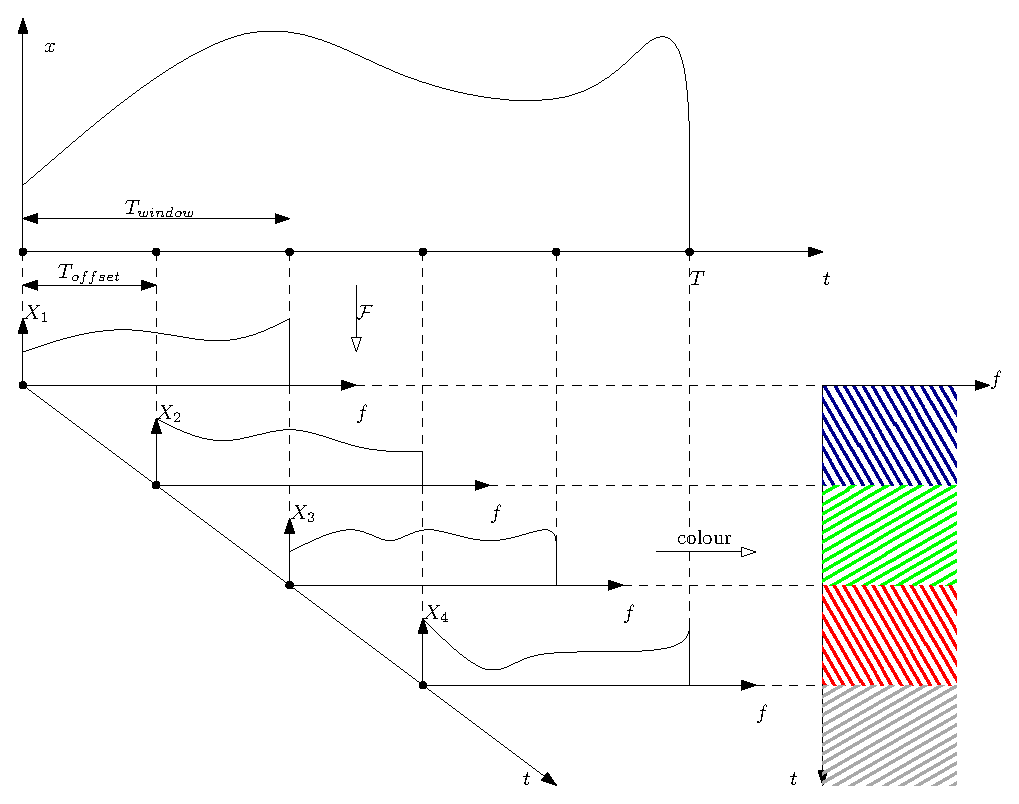
\includegraphics{drawings/spec.eps}
				\caption{The process of creating a spectrogram.}
				\label{fig:spec}
			\end{figure}

	\subsubsection{Principal Components Analysis}
		Here we present the theory for Principal Components Analysis (PCA) based on Andrew Ng's lecture notes \cite{ng13} and Kevin Murphy's book \cite{mlBook}. The objective is to take $m$ $n$-dimensional input data points $\{\vec x^{(i)} \in \mathbb{R}^n\}_1^m$ and transform them into $m$ $k$-dimensional data points ($k<n$) $\{\vec y^{(i)} \in \mathbb{R}^m\}_1^m$, where $\vec y^{(i)}$'s are projections of $\vec x^{(i)}$'s onto $k$ orthonormal basis vectors $\{\vec u_i\}_1^k$ while ``preserving the most variance''. We assume that over all $m$ points, their $\text{mean}\left[\{x^{(i)}_j\}_{i = 1}^m\right] = 0$ and their $\text{var}\left[\{x^{(i)}_j\}_{i = 1}^m\right] = 1$ for all features of the input points $1 \leq j \leq n$. We normalise the data first if this is not the case. For $n = 2$, $k = 1$, Figure \ref{fig:pca} shows the projections to the new axis.
		\begin{figure}[h!]
			\centering
				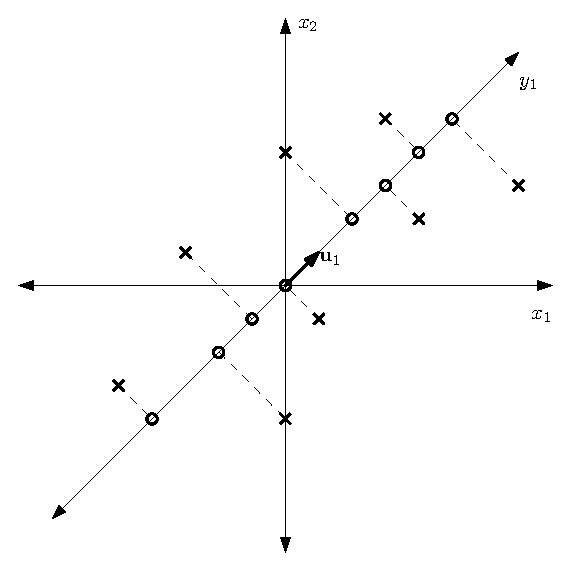
\includegraphics{drawings/pca.eps}
			\caption{Illustration of PCA.}
			\label{fig:pca}
		\end{figure}

		We can see that the transformed points can be expressed as
		\begin{equation}
		 	\vec y^{(i)} =
		 		\begin{bmatrix}
		 			\vec u_1^T \vec x^{(i)} \\
		 			\vec u_2^T \vec x^{(i)} \\
		 			\vdots \\
		 			\vec u_k^T \vec x^{(i)} \\
		 		\end{bmatrix}
		 		, 1 \leq i \leq m
			\label{eqn:pca}
		\end{equation}
		
		It can be shown that in order to maximise $\sum_{i = 1}^m \left\| \vec y^{(i)} \right\|^2$, conditioned on orthonormality of the bases, we must choose normalised eigenvectors corresponding to the $k$ largest eigenvalues of the variance matrix $\vec \Sigma = \frac{1}{m} \sum_{i = 1}^m \vec x^{(i)} {\vec x^{(i)}}^T$ as the bases. These bases are also called the \emph{principal components}. The eigenvalues are proportional to the actual variances of data in the new bases. Hence, we can compare the relative ``importance'' of the bases and use this fact to decide how many principal components to use.

\newpage
\section{Machine Learning -- Experiments}

\paragraph{}
	We obtained the data from the ECG database from the PhysioNet database located at \url{http://physionet.org/physiobank/database/apnea-ecg/}. The data consists of 35 labelled training records and 35 unlabelled records (used for the CinC Challenge 2000 competition). The recordings vary from less than 7 hours to 10 hours each and include continuous digitised ECG signal and, in the case of the training data, a set of apnoea annotations derived by human experts. The continuous signal is sampled at the rate of 100 Hz and the annotations are available at every 6000 samples (i.e. every minute) of the signal indicating the presence of apnoea at that time. One such record is shown in Figure \ref{fig:visualiseData}.

	\begin{figure}[ht!]
		\centering
			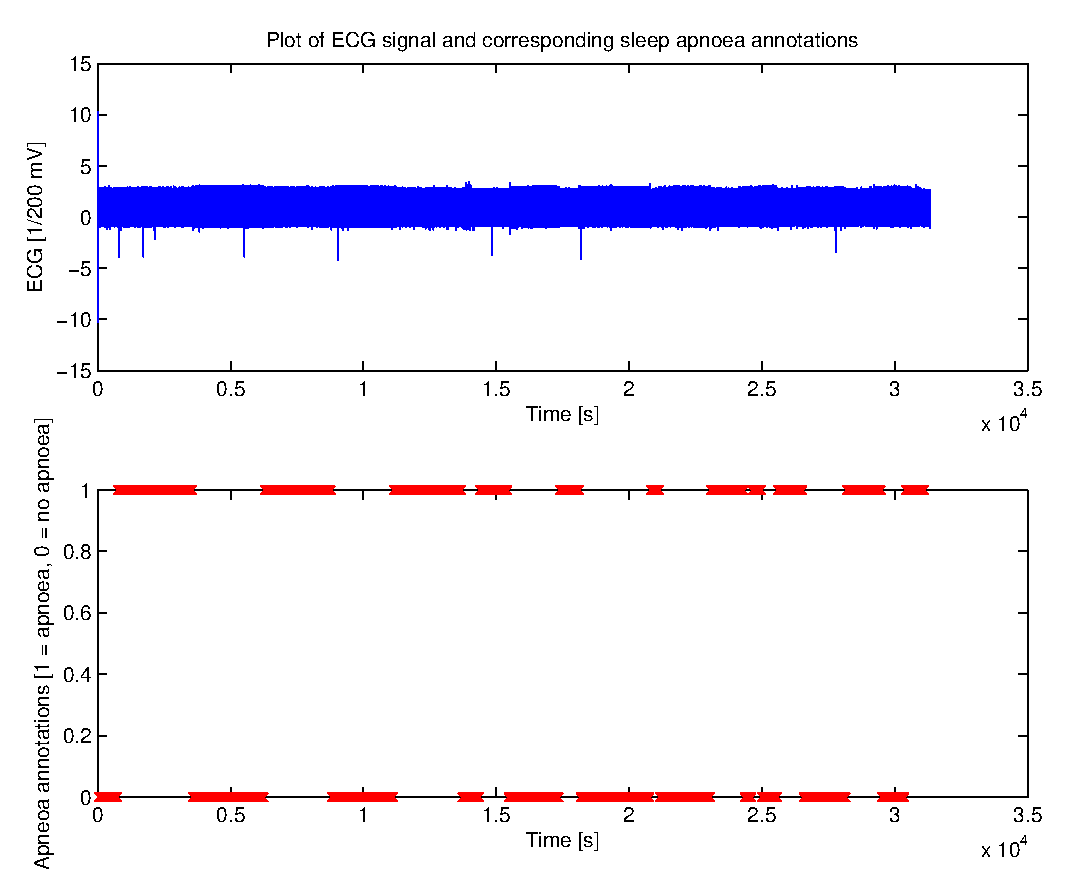
\includegraphics{drawings/visualiseData.eps}
		\caption{One training record}
		\label{fig:visualiseData}
	\end{figure}

\subsection{Conditioning input data}
\label{sec:conditioningExperiments-ta}

\subsubsection{Frequency Analysis}
	We use \verb!MATLAB!\textsuperscript{\textregistered}'s function \verb|spectrogram|, which takes the following parameters
	\begin{itemize}
		\item \verb!X! -- our signal $\vec x = \{x_1, x_2, \dotsc, x_N\}$.
		\item \verb!WINDOW! -- length (in number of samples) of the window $T_\text{window}$. The windows are automatically filtered using a Hamming window. We arbitrarily choose the window to be the number of signal samples corresponding to one annotation (6000 in our case).
		\item \verb!NOVERLAP! -- number of overlapping samples between two consecutive windows. Effectively $T_\text{window} - T_\text{offset}$. We arbitrarily choose the offset to be 1000 such that we have six bins of PSD's for each annotation.
		\item \verb!NFFT! -- number of frequency points used to calculate the discrete Fourier transforms. We use default.
		\item \verb!Fs! -- sampling frequency in Hz. In our case 100 Hz.
	\end{itemize}

	A spectrogram for one record can be seen in Figure \ref{fig:visualiseSpectrogram}. Just by looking at the spectrogram, we can spot different regimes of the time series (most clearly seen at $0.5 \times 10^4$, $1 \times 10^4$, $2 \times 10^4$, and $2.7 \times 10^4$ seconds). Comparing this to the apnoea annotations in Figure \ref{fig:visualiseData}, these regimes are actually the non-apnoeatic regimes. Also, we can see that most of the ``action'' is happening below 20 Hz. For this reason, we cut off the frequencies above 25 Hz for subsequent analysis. We combine the corresponding six bins of PSD's per annotation in to a large feature vector corresponding to that annotation. The actual implementation can be found in Appendix \ref{sec:transformSpectrogram}. Next, we will reduce the dimensionality of these feature vectors using PCA.
	\begin{figure}[ht!]
		\centering
			\includegraphics[width=.5\textwidth]{drawings/visualiseSpectrogram.eps}
		\caption{Spectrogram of one record}
		\label{fig:visualiseSpectrogram}
	\end{figure}

\subsubsection{PCA}
	For this, we use the function \verb!pca! from the package \verb!pmtk3!. Once we get the principal components (orthogonal bases) and their corresponding principal coefficients (variances of the data, projected onto that base, correct to a constant factor) $\{\lambda_1, \lambda_2, \dotsc, \lambda_D\}$, we will plot the graph of their cumulative sum over their total sum $\frac{\sum_{i = 1}^n \lambda_i}{\sum_{j = 1}^N \lambda_j}$ in order to decide on the number of principal components needed. The plot is in the Figure \ref{fig:visualisePca}. Performed on the first 10 records, we can see that we will need to include at least 100 to capture half of the variance but at least 3000 components to capture the whole variance. The actual implementation can be found in Appendices \ref{sec:pcaCalc} and \ref{sec:pcaTransform}.
	\begin{figure}[ht!]
		\centering
			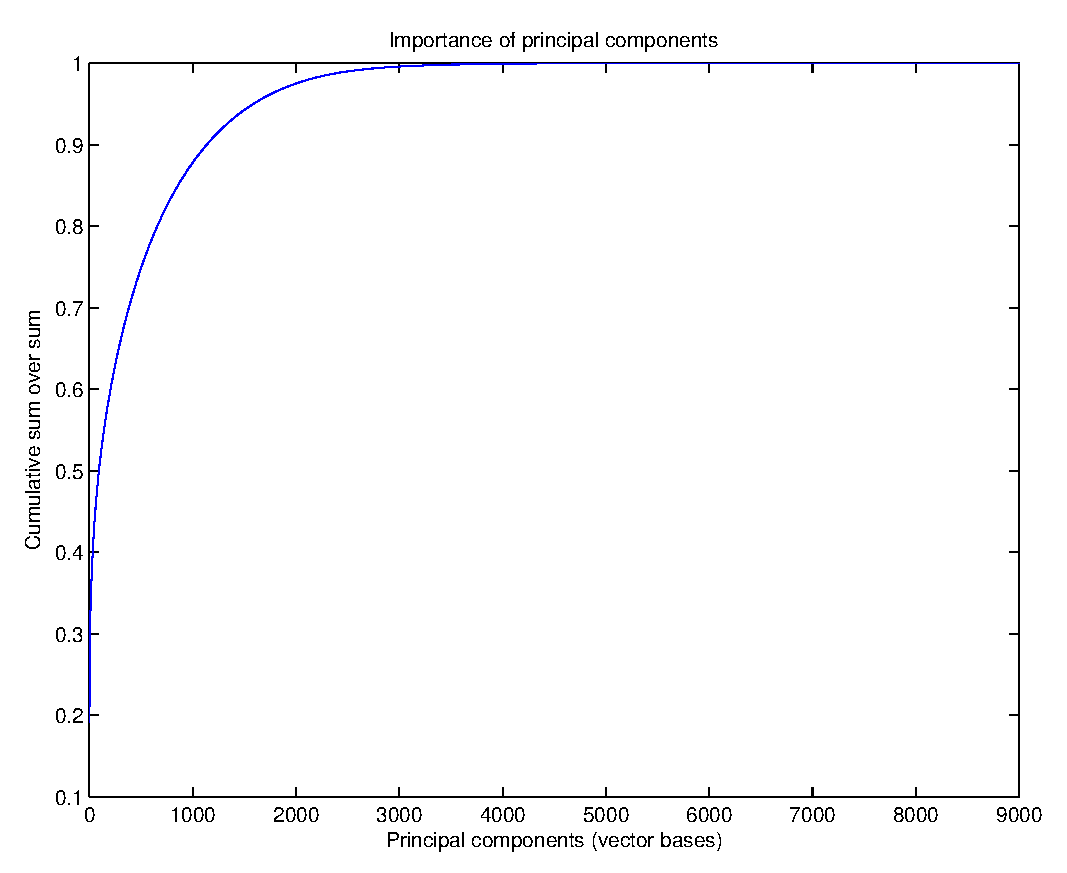
\includegraphics[width=.5\textwidth]{drawings/visualisePca.eps}
		\caption{PCA of the first 10 records}
		\label{fig:visualisePca}
	\end{figure}
\subsection{Data Visualisation}  
\subsection{Support Vector Machines}
\subsection{Hidden Markov Models}

Having examined briefly the theory behind Hidden Markov Models, let us now look at how the training was done offline, and analyse some results from subsequent tests. As mentioned earlier, the apnoeatic states are modelled as the hidden states $\{x_t\}_1^T$, and are elements of the binary set $\{0, 1\}$. The observed signal is annotated every K samples (every minute in the case of the PhysioNet data), so we stack all K samples into $\vec y_t \in \mathbb{R}^d$, ($d = K$). Using the packages \verb!pmtk3! and \verb!HMM Toolbox!, the algorithms were implemented in \verb!MATLAB!\textsuperscript{\textregistered}, along with the conditioning of the data using spectrogram and PCA analysis. Again, \verb!MATLAB!\textsuperscript{\textregistered} is used for convenience and the code can be easily converted to \verb!Java! after experimentation and analysis.

We present below parts of the code used for the training and testing of the data, for ease of explanation. Firstly, we present the main script, covering the reading and conditioning of data, spectrogram transformation and PCA analysis. After explaining the various functions created and used in the script till then, we move on to cover the training and testing of the data.

\begin{lstlisting}
trainIndex = 1:10;
testIndex = 11:15;

%% Reading and conditioning data
[Y, X] = readData(trainIndex, 0); % Y = observations, X = latent states.
N = 2; % number of states: apnea-noapnea
S = [0; 1]; % set of possible states

%% Transform spectrogram
[YTransformed, XTransformed] = transformSpectrogram(Y, X);

%% PCA
disp('PCA...');
k = 100; % take k principal components only
[PCoef, PVec, YMean, YVar] = pcaCalc(YTransformed, k);
figure;
plot(cumsum(PCoef)/sum(PCoef));
YPca = pcaTransform(YTransformed, PVec, YMean, YVar);
\end{lstlisting}

The trainIndex and testIndex vector are used simply for selecting the files to be used, out of 35, for training and the remainder (or less) for testing the accuracy of the diagnosis. Having chosen the files, the next step is to extract and read the files. This is done using the readData function, presented below:

\begin{lstlisting}
function [O, q, time, signal, annTime] = readData(fileIndex, keepSignal)

    disp('Reading and conditioning data...');
    filenames = getFilenames();

   % Initialise Variables (not shown)

    for i = fileIndex
        filename = cell2mat(filenames(i));
        disp(sprintf('\tProcessing file %d: %s...', i, filename));
        
        [timeTemp, signalTemp, freq] = rdsamp(filename); % reads the signal
        [annTimeTemp, type] = rdann(filename,'apn'); % reads annotations
        type = (type == 'A');

        %% Conditioning data
        annTimeTemp = [1; annTimeTemp];
        q = [q; type]; % latent states
        for i = 1:length(type)
            O = [O; signalTemp((annTimeTemp(i) + 1):annTimeTemp(i + 1))'];
        end
    end
end
\end{lstlisting}

The function reads data from the indices specified in fileIndex (which is trainIndex in the main script above), and returns O, containing all the observations merged together in a TxD matrix. T is the total number of minutes of data, and D is the number of samples in a minute (6000 in this case), such that there are T annotations in total. The function also returns the vector q, a Tx1 vector containing the latent states for every minute in O, as well as consolidated time, signal and annotation time vectors for ease of plotting and analysis later on.

Firstly, readData uses a simple function getFilenames to return a 35x1 cell of the available filenames, in a cell string. Then, after initialising the variables, readData uses a for-loop to run through each file and extract the relevant information. Using the pre-provided rdsamp and rdann functions, the signal values as well as annotations are read from the file. As the annotations use 'A' for apnoeatic episodes and 'N' for non-apnoeatic episodes, the vector type is converted to the alphabet ${0,1}$. The O and q output matrices are built up using the information from each file, and finally some trivial conditioning is done to ensure ease of plotting if the signal were to be kept.

Armed with the consolidated vectors X and Y, we now proceed to use the spectrogram function in \verb!MATLAB!\textsuperscript{\textregistered}, as described in section~\ref{sec:conditioningExperiments}. We then use the \verb!pca! function from the \verb!pmtk3! package to perform Principal Components Analysis (choosing the number of principal components we wish to include, k). 

We then move on to training and fitting the parameters, using the \verb!pmtk3! and \verb!HMM Toolbox! packages. We then compare the expected hidden states calculated using the \verb!Viterbi Algorithm! with the actual underlying states and determine the accuracy of the HMM model diagnosis.
\begin{lstlisting}
%% Fitting parameters
[A, Mu, U, pi] = apneaHMM4Train(XTransformed, YPca, N, S);

%% Comparing with test data
apneaHMM7Test(A, Mu, U, pi, PVec, YMean, YVar, N, testIndex);
\end{lstlisting}

The parameters are fitted using the apneaHMM4Train function shown below (the number 4 simply represents the final version that we used), which computes the transitional matrix A using
\begin{align}
		A_{ij} & = \frac{\sum_{t = 1}^{T - 1} 1\{x_t = s_i \land x_{t + 1} = s_j\}}{\sum_{t = 1}^{T} 1\{x_t = s_i\}}
\end{align}
and uses Gaussian fitting to calculate the pdfs for the emissions (the gaussFit function is used from the \verb!HMM Toolbox! package - we shall not go into the details on how the function is implemented here). We are left with the outputs A, the 2x2 transition matrix, Mu and U, parameters of the Gaussian pdf fit of the emissions, and pi, the initial state distribution.
 
\begin{lstlisting}
function [A, Mu, U, pi] = apneaHMM4Train(q, O, N, S)
    [T, D] = size(O); % dimension of observations & number observations

    % Transitional matrix A
    disp('Fitting transitions...');
    A = zeros(N);
    for i = 1:N
        for j = 1:N
            transitionsFromSiToSj = 0;
            transitionsFromSi = 0;
            for t = 1:(T - 1)
                transitionsFromSiToSj = transitionsFromSiToSj + (q(t) == S(i) && q(t + 1) == S(j));
                transitionsFromSi = transitionsFromSi + (q(t) == S(i));
            end
            A(i, j) = transitionsFromSiToSj / transitionsFromSi;
        end
    end

    % Estimate Gaussian parameters
    disp('Fitting emissions...');
    Mu = zeros(D, N); % means
    U = zeros(D, D, N); % covariances
    for j = 1:N
        x = O(q == S(j), :);
        model = gaussFit(x);
        Mu(:, j) = model.mu;
        U(:, :, j) = model.Sigma;
    end

    % Estimate HMM parameters
    pi = [0.5; 0.5];
end
\end{lstlisting}

In order to compare with the test data, we need to read the data specified using the testIndex, condition it, and use the \verb!Viterbi Algorithm! to calculate the most likely path. This is done in the function apneaHMM7Test, shown below. The code for reading and conditioning the data (and plotting the results) has been ommitted as it is similar to that shown above. Once again, functions from `off-the-shelf' packages are used in implementing the \verb!Viterbi Algorithm! and the accuracy of the most likely path is calculated by comparing it to the annotations reflecting the true states. This is done for each test file, and the results are shown below.  

\begin{lstlisting}
function apneaHMM7Test(A, Mu, U, pi, PVec, OMean, OVar, N, testIndex)
    disp('Comparing with test data...');
    accuracySum = 0;
    for i = testIndex
        %% Read data
        %% Transform spectrogram
        %% PCA

        %% Most likely path (Viterbi)
        disp(sprintf('\tCalculating the most likely path...'));
        B = [];
        for j = 1:N
            B(j, :) = gaussian_prob(OTest', Mu(:, j), U(:, :, j));
        end
        path = viterbi_path(pi, A, B) - 1;
        
        accuracy = sum(path == qTest') / length(qTest)
        accuracySum = accuracySum + accuracy;
        
        %% Plotting data
    end
    avgAccuracy = accuracySum / length(testIndex)
end
\end{lstlisting}

The results for the HMM experiment are shown in Figure \ref{fig:hmmExperiment}. While the average accuracy is much lower than that found for the SVM model, at 64.1\%, we feel that the HMM model would still be more appropriate than the SVM one due to the absence of Support Vectors which tend to lead to poor generalisation performance. Due to limited time and computational power (fitting the parameters takes a considerable amount of time on a standard laptop), we were unable to utilise the full set of data for our experiments. However, we are confident that if more time and effort were to be expended in this area, the HMM model would prove to be more accurate in diagnosing apnoea as compared to the SVM model. This is because of the suitability of the Hidden Markov Model for temporal data and the applicability of the Markov assumptions in our case.

\begin{figure}[ht]
		\centering
		\subfloat[record 11]{%
			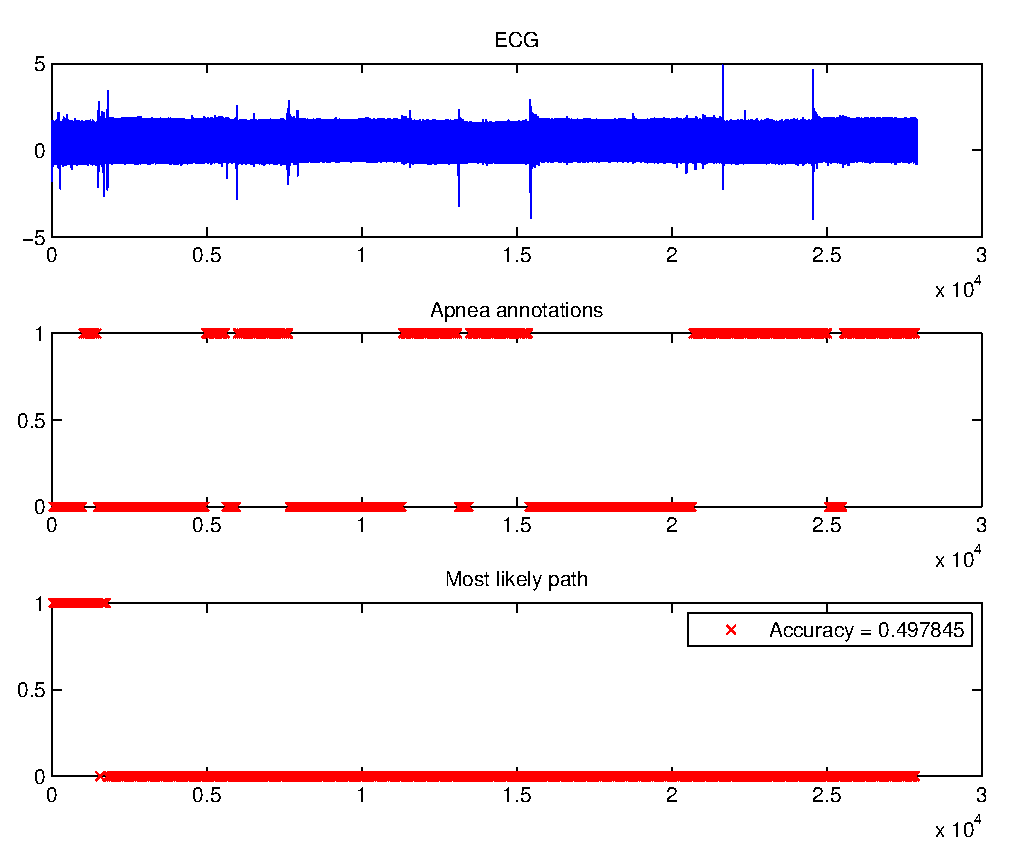
\includegraphics[width=.33\textwidth]{drawings/hmm/hmmTest11}}
		\subfloat[record 12]{%
			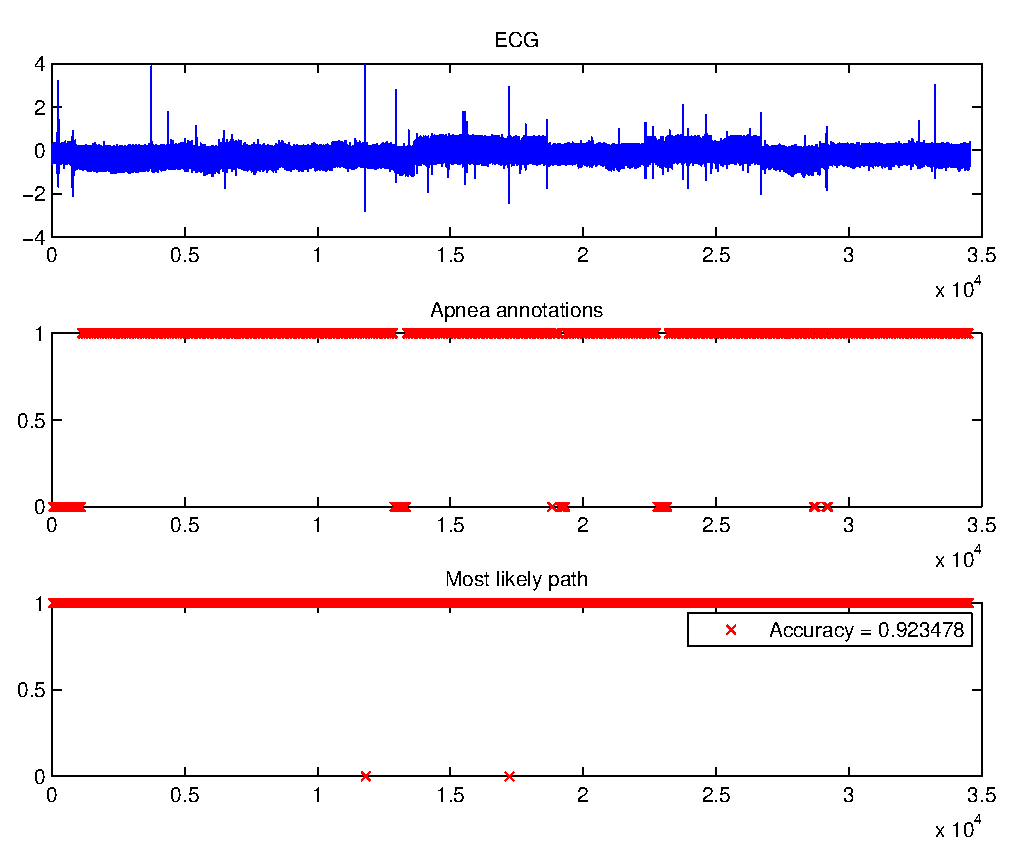
\includegraphics[width=.33\textwidth]{drawings/hmm/hmmTest12}}
		\subfloat[record 13]{%
			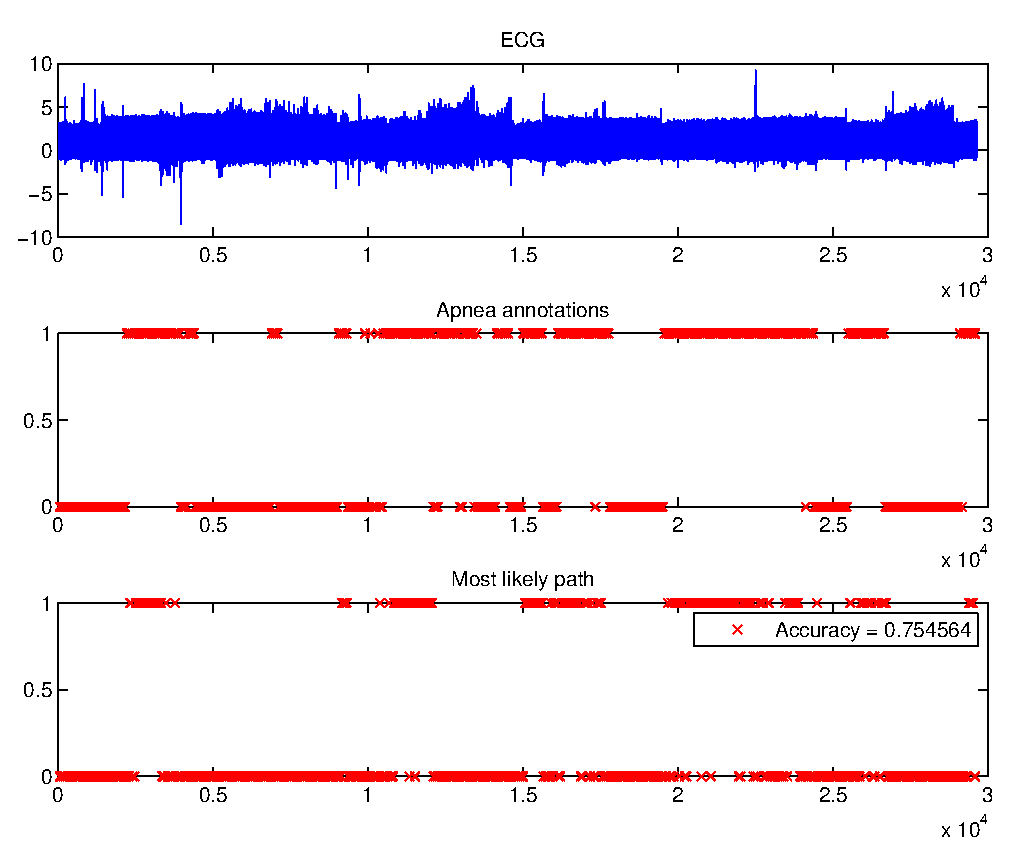
\includegraphics[width=.33\textwidth]{drawings/hmm/hmmTest13}} \\
		\subfloat[record 14]{%
			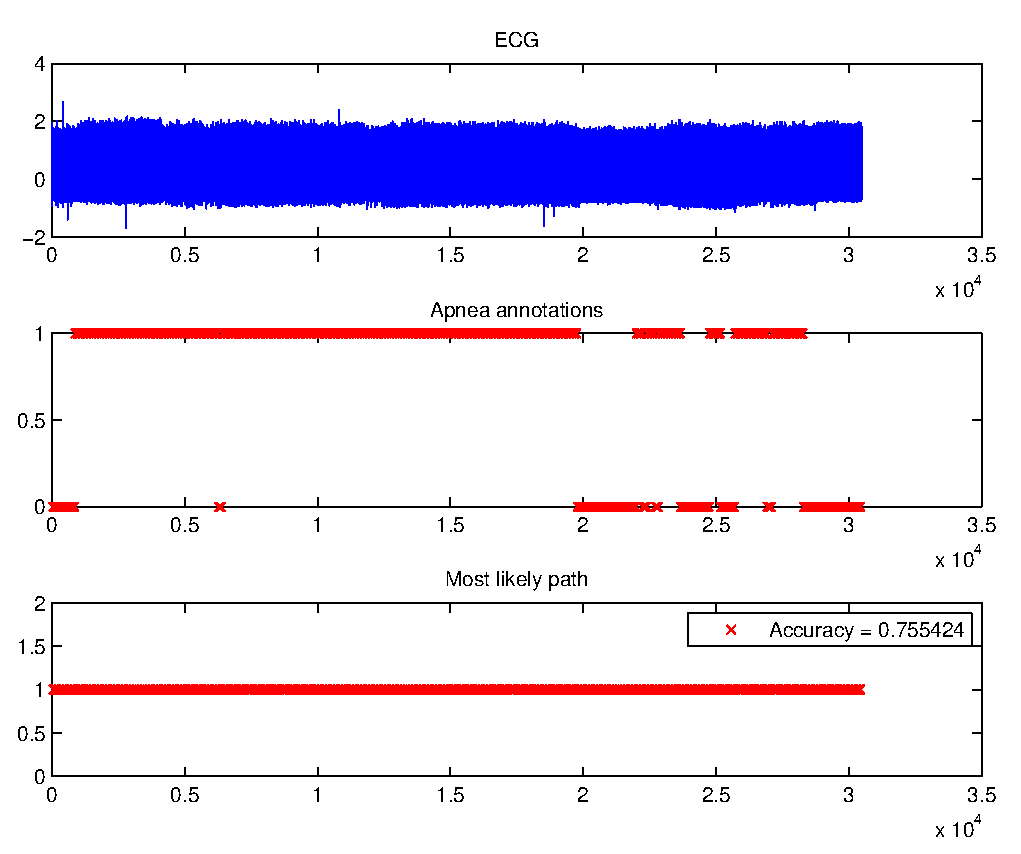
\includegraphics[width=.33\textwidth]{drawings/hmm/hmmTest14}}
		\subfloat[record 15]{%
			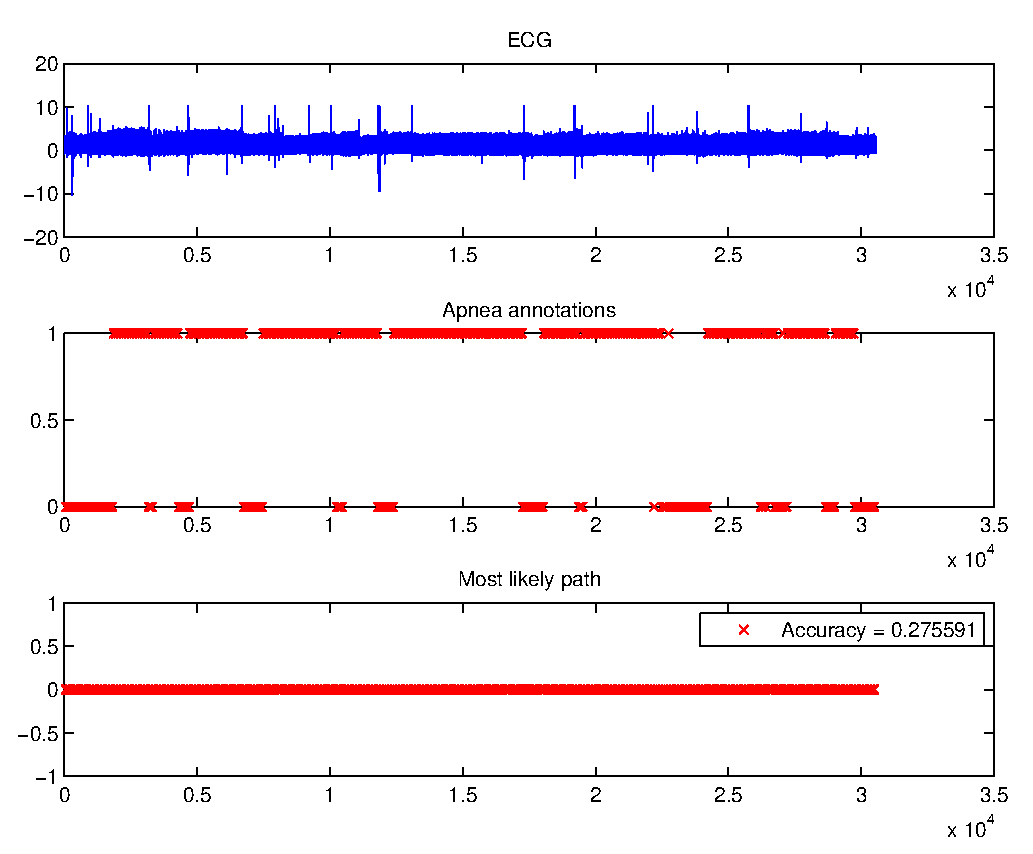
\includegraphics[width=.33\textwidth]{drawings/hmm/hmmTest15}}
		\caption{Performance of HMM model on the test records 11 to 15}
		\label{fig:hmmExperiment}
\end{figure}

\subsection{Summary}
\label{sec:mlExperimentsSummary}

We have seen the implementation of the SVM and HMM models to the PhysioNet data and have calculated the accuracy of both methods in diagnosing apnoea from five records. On the surface, while it may seem that the SVM model provides us with higher accuracy, we feel that the HMM model is more appropriate for use in our app. The accuracy can be improved, firstly, by using more data (we only used 10 of the 35 files for testing) and secondly, by ensuring that the annotations on training and testing data reflect the reality of the patient.

What we have managed to prove here, however, is that diagnosis of OSA using non-invasive techinques is possible if the appropriate machine learning tools are utilised. If more resources were to be invested, an accurate and comprehensive diagnosis can be created in conjunction with the questionnaire.

\newpage
\section{Machine Learning -- Java}

\newpage
\section{Designing an Android App (George)}
\label{sec:android-george}
In this section of the report about designing an Android app with the “Android Developer Tools” (ADT) software, there will not be any coding guidance on the basics of Java nor XML. As such, any examples discussed or shown will either have a short explanation or will be simple enough to assume the functionality of the code is evident. The ADT software is used in this project as it facilitates the balance in a simple to use package yet includes more detailed app functionality such as accessing the sound recorder’s buffer. There are many other Android app developing software packages, but none achieve this balance as well. For example the “MIT app inventor” provides basic building blocks for an app but limits the customisation of the code that is an essential element for our audio processing. “appsgeyser.com” is even simpler in providing an app interface for a pre-existing website. However we have decided not to use a web-based approach due to the extra complications from patient security and limitations in excessive data usage in streaming audio to a website.
\subsection{XML and Java sides of ADT}
The “Android Developer Tools” software has a simple architecture for basic apps, which uses XML code to create the user interface of buttons and graphics, and Java code to describe to the phone what each of these items in the XML code does. So for any page of the phone app, there is an XML code called the “layout” with an associated set of Java instructions called a Java “activity”. Whilst it is intuitively easier to consider a visual layout with instructions behind each section, the programming design works much more naturally the other way around, with the Java activity dictating the layout. For this particular app, we need four pages in total. Therefore we need to create a total of four Java activities to describe each page, and each one of these will call an XML layout to attach various commands to.
\subsection{XML IDs}
Each interactive item of the XML layout will have a unique ID, and the Java code will directly link an object to this, which can then be used in the functionality instructions. The following code first assigns the XML button ID “btn\_analyse” to a Java button object called 'btnAnalyse', then informs the phone to carry out the task “startAnalyseActivity()” when it detects that the button has been pressed.
\begin{lstlisting}
btnAnalyse = (Button) findViewById(R.id.btn_analyse);
btnAnalyse.setOnClickListener(new View.OnClickListener() {
public void onClick(View v) {
startAnalyseActivity();
          }
    });
\end{lstlisting}
Our application uses a minimalistic interface and as such there are few XML IDs to work with. Regardless, a convention was established such that each object is labeled by it’s type followed by an underscore, then it’s unique name (for example btn\_analyse as above).
\subsection{Methods}
The task “startAnalyseActivity()” used in the example above is known as a “method” in Java code and is a set of code instructions grouped together under a single name. Not only does this make the code clearer to understand, it also allows repeated sections of code to be called much more simply: just contain all the repeated parts under one method and call that method each time. For these reasons, code for each part of the application functionality is contained in separate methods.
\subsection{Java and android libraries}
The app writer is not expected to write machine level code for the smart phone and is provided with a large array of building blocks for both Java and Android based coding which are contained in “libraries” which must be imported at the start of each activity. For example, the “Android.media.AudioRecord” library is needed to use the phone’s built in microphone, and it provides simple inbuilt methods such as “startRecording()” and “stop()”. Further details of this particularly important library will be discussed later.
\subsection{Structure of an Activity}
Each activity can be divided down into several key blocks that can be explained in the chronological order in which they are seen in the code:
\begin{enumerate}
\item Importing the necessary libraries of methods
\item Declaring the whole activity to create it
\item Declaring any variables and objects that the activity uses
\item Creating the onCreate() task upon which the activity starts running, and in which the core instructions and external methods are called
\item Defining any extra methods used, with their code detailed inside
\end{enumerate}
\subsection{XML writing}
Again, it is not within the scope of this report to comprehensively explain how to code XML, but the code here is very clear to comprehend upon reading each line of code. The “Android Developer Tools” software allows the user to directly edit the XML code, and to also view and edit the layout from a graphical “preview” layout. Note that editing either one of these will update the other in real time. Each object is defined in a block enclosed by < and /> and must contain it’s own ID definition as a minimum. The app’s theme will dictate a large set of default values for any object parameter, so only the physical size and details unique to each object need to be added. This might include unique text for a button or a variation in font for some text – all of which are edited under very clear labels such as “android:fontFamily=…”.
\subsection{XML layouts}
The overall page layout has two main formats: linear layout and relative layout. Relative layout requires each object’s relative position to be labelled in reference to at least one other object with a fixed location and allows objects to be placed alongside each other as well as above and below (effectively two dimensions of freedom). Linear layout is simpler and more constrained in that the objects will be placed in the order they appear in the XML code in one dimension. For this application, linear layout is suitable. Other useful tools here include “<ScrollView/>” which allows all objects within it to be viewed as a scrollable page. This was used on the questionnaire to prevent the questions becoming too small to be readable. It can also be used internally to scroll a subset of objects rather than the whole page.
\subsection{Further XML details}
When defining an object’s size, it’s useful to use adaptable sizes to ensure good results on all devices and screen sizes (as opposed to a set height of 10px for example, which could look small on a tablet but large on a small phone). The two options here are FILL\_PARENT, which makes the object as wide as the object it’s contained in, and WRAP\_CONTENT, which makes the object as wide as necessary to contain all of its components. Using the example of a button width inside an empty android page, FILL\_PARENT would make the button as wide as the screen, and WRAP\_CONTENT would make the button wide enough to include all the button text.
\subsection{Handling Strings}
When creating buttons and other features with text on, the text should be stored in the separate file in “res/values/strings.xml” instead of ‘hardcoding’ it directly into the XML code. Whilst it is less of an issue on a small-scale project such as this, it can become increasingly difficult to find where to change particular items of text in larger projects. Instead we label each part of text from the strings file and reference this ID where it is needed in the code. Then we can quickly find where to change any text in future, or perhaps reuse the same text in multiple buttons or other applications.
\subsection{Java Techniques}
Sharing data between activities can be achieved with a basic technique called “SharedPreferences” which stores any required variable locally in the app. As with many techniques, it requires importing its own class from the android library, and vitally requires the command “editor.commit()” to save the changes before finishing. It is utilised in this application to store the received information from the questionnaire. By restoring the previous stored settings upon the app initialisation, the questionnaire results are then stored on a more permanent basis (I.E when the application has been closed and reopened).
\\ Changing from one activity to another is done using a class called “Intent” which is effectively setting up a requirement for something to happen. In this case the intent will provide the details of the activity to be launched. A button press might then call “startActivity(intent)” which will launch whatever the original intent requested. In this way it can be used as an independent launching mechanism as it is not aware of the details of the intent nor is the intent solely aimed at one target. For example, multiple buttons can launch one action, all acting as effective triggers. In this application, intents are primarily used to launch new activities.
\\ When starting multiple activities, care needs to be taken as to how and when previous activities are closed. Whist it might seem to make sense to have the home page close upon opening a new window, this posed a subtle bug in practice. The pressing of two activity-launching buttons simultaneously causes both of them to open and this is not a significant issue. However, pressing the back button in this format requires launching the “home page” again. Therefore upon exiting one page, a residual page is left open behind the current home page, and upon a few repetitions of this, the app will quickly be running several pages simultaneously. Without exploring in too much depth how to make each activity-launching button press a unique event (such as a mutex-like control), the simplest solution in this case was to allow up to three of the new activity pages to open simultaneously and leave the “home page” unclosed. This limits the total possible number of pages open to four. This is a very unlikely event, and is easily remedied by pressing the back button.
\\ “RadioGroup” buttons are used in the questionnaire section of the app. These provide the advantages of never leaving a blank answer and being instantly comprehendible to any user. Similarly to the buttons, each one has a unique ID to be linked with the Java activity, but they also have unique IDs for each possible selection. The selected answers can then be acted upon by ‘if’ statements using:
\begin{lstlisting}
if (radioOne.getCheckedRadioButtonId() == R.id.radioY1)
  { /* Do action */ } 
\end{lstlisting}
\subsection{Initialising AudioRecord}
It is worth looking in further detail at the AudioRecord android class that we use for the audio input. The initialisation of “new AudioRecord()” uses five parameters, which are explained below:
\begin{itemize}
\item “audioSource” should be set to “1” to default to the inbuilt microphone
\item “sampleRateInHz” should be set to “44100” to guarantee functionality on all devices, however a much lower sample rate would be preferable for the basic application here, and a solution to this is described below.
\item “channelConfig” should be set to “16” for recording sound in MONO rather than STEREO. 
\item “audioFormat” should be set to “2“ for PCM 16bit or “3” for PCM 8bit. This application uses 16bit to ensure functionality on the greatest number of devices possible.
\item “bufferSizeInBytes” is set using an inbuilt method called “getMinBufferSize()”. The inputs to this are the same as parameters 2, 3 and 4 in the AudioRecord initialisation.
\end{itemize}
So the initialisation for the application should look as follows:
\begin{lstlisting}
new AudioRecord(1,44100,16,2,getMinBufferSize(44100,16,2));
\end{lstlisting}
In practice, each input is assigned to a variable that is defined at the top of the code for easy modification and better clarity in the code.
\\ For recording snoring frequencies, a sample rate of as low as 4000Hz would be adequate. The following code solves the earlier discussed issue of minimising the sampling rate. The “getMinBufferSize() is tested on each value added in the for() loop, but as soon as the function returns a positive (hence a valid) bufferSize, the method returns this lowest valid sample rate and “breaks” to finish the method.
\begin{lstlisting}
public int getValidSampleRates() {
  int samplerate = 0;
for (int rate : new int[] {8000, 11025, 16000, 22050, 44100}) {
  int bufferSize = AudioRecord.getMinBufferSize(rate, AudioFormat.CHANNEL_CONFIGURATION_DEFAULT, AudioFormat.ENCODING_PCM_16BIT);
if (bufferSize > 0) {
  samplerate = rate;
  break;}
}
return samplerate };
\end{lstlisting}
\subsection{Progress Wheel}
A progress wheel requires two tasks to be carried out simultaneously – the wheel itself, and the task that has the progress being indicated. This is done with the AsyncTask that allows a background operation to interact with the user interface element: effectively two threads are running and we can allow the UI thread to be updated from the background task. There are four self-explanatory steps in the asynchronous task called onPreExecute, doInBackground, onProgressUpdate and onPostExecute.
\\ To use an example in this app, the “SaveToFileTask” first calls the progress wheel to show on screen with “ProgressDialog.show(…)” in the onPreExecute() step. It then calls the method “audioData.saveData(…)” in the doInBackground() step and finally calls “progressDialog.dismiss()” in onPostExecute() which will clearly indicate that the data has been saved. Note that the onProgressUpdate step is not used, as we do not have a use for updating the UI whilst running the background task. This might, for example, be used to change the text on the progress wheel to indicate when a second task is being carried out had one been present.
\subsection{GraphView}
GraphView is an additional library available for Android and is particularly useful for an audio application that looks at sound intensities. 
\subsection{Other Platforms}
Apple provide their own libraries similar to those in android, that provide quickly usable methods and hardware capability to a developer. The sleep apnea app has suitably simple components that can be recreated on Apple’s iOS like for like if required. This section of the report will quickly overview the techniques to do this, but will also detail other available tools and how they might be used more to create a more effective native app in iOS. This section will not detail any code, purely discussion of the available libraries and tools.
\subsection{Xcode}
Xcode is the free software available in the Apple App Store that contains all the necessary prototyping and developing tools to produce an application on iPhone, iPad and Mac. Code can be written in Objective-C, C and a whole multitude of other languages with interpreters to adapt them. Xcode provides an Integrated Development Environment (IDE), compiler with inbuilt “bug” finding, an iOS simulator to virtually test the app amongst other things. Similarly to the Android Developer Tools, memory analysis, CPU profiling and general performance tracking is all included. This would provide a very suitable basis to build our app from.
\subsection{AVAudioRecord Library}
The most important library to consider here is the inbuilt capabilities of the audio recording. A handful of the more unique and interesting classes will be discussed here:
\begin{itemize}
\item recordAtTime:forDuration: This flexibility in setting the start time to record and the duration of each recording could be applied for a few things. Firstly the start time could be set such to greatly increase the chance of the user being asleep as the recording starts. It could also be used as a basic way to reduce background noise if, perhaps, the user’s sleeping area experienced background noise from parties or traffic until a set time in the evening. Likewise, limiting the duration of the recording could ensure results aren’t skewed from noise of waking up and manually turning the app off. The app could select a key range of hours in the night that maximises the probability of apnea detection and minimises the chance of background noise. Note that this could also be manually implemented in the Android version which is discussed later.
\item averagePowerForChannel This is one of two values provided in the Audio Level Metering section of the library. This could provide a very simple technique to implement a switching state model with perhaps three defined ranges of audio powers. Recording the average power for the channel (in our case there is only one channel in MONO recording) roughly twice per second would provide an array which would accurately reflect the volume of the sleeping user. “Band two” would represent the standard snoring volume observed in almost all sufferers of sleep apnea and would be the expected volume level for the user. “Band one” would be very low audio power indicative that the sleeper’s throat is blocked and an apnea is occurring. “Band three” would represent high audio power, interpreted as the loud snorting very commonly experienced after an apneic episode as the sleeper unblocks their throat. Clearly such a monitoring system would produce very small file sizes, which is a very desirable aim in audio recording based software (in this case, audio isn’t being saved directly to a file, only monitored for power values). This technique doesn’t lend itself well to machine learning techniques due to the lack of precision in the recorded data – features aren’t defined nearly as well as more fully sampled techniques.
\item peakPowerForChannel is the other value provided by the Audio Metering section and whilst not being as directly applicable, could be useful when used in conjunction with averagePowerForChannel. From simple logical reasoning, noise is much harder to detect when the precision of the system is low like the technique suggested above. peakPowerForChannel could therefore be used to calibrate this technique. A short recording of the background noise in controlled quiet conditions could calibrate the allowable background noise for “band one” in the above example, whilst the user recording a faked snort sound could provide a rough expectation for the power to be expected at “band three”. From this, unexpected audio power levels can be rejected or handled differently from the normal operational audio power.
\end{itemize}
\chapter{Conclusion (Sachin)}
\label{ch:conclusion}
 
Obstructive Sleep Apneoa (OSA) is a serious and prevalent condition that affects many middle-aged people, and many of them remain undiagnosed, leading to poor sleep and a reduced quality of life. The current diagnosis solutions offered by the NHS are relatively expensive and inconvenient, and there is a need in the market for a way to check for OSA without having to spend a lot of time, money or effort. The easiest way to provide for this need would be through a smartphone application that would utilise machine learning to diagnose OSA from the user's audio sleep data.

After proving that there is a need and potential market for a mobile app that is able to provide a preliminary diagnosis of OSA, we moved on to first develop a method of diagnosis without using machine learning, to use as a backup and to familiarise ourselves with sleep data. We created a simple method of diagnosis in \verb!MATLAB!\textsuperscript{\textregistered} using power thresholds and variance analysis. This method was able to provide us with an output of 1s or 0s, highlighting different time periods when the user experiences apneoa. We then tested the simple method on a 7 minute audio file obtained from the internet, of a real OSA patient.

We then moved on to research several machine learning techniques that could be used in our app, and identified Support Vector Machines (SVM) and Hidden Markov Models (HMM) as being suitable in our case. We built the models in \verb!MATLAB!\textsuperscript{\textregistered} and ran tests using data obtained from PhysioNet to test the accuracy of both models. We presented the results and argued in Section \ref{sec:mlExperimentsSummary} that the HMM model would be better suited for the purpose of diagnosing OSA from temporal data. 
More importantly, what we were able to show was that if the appropriate model is used, OSA can be accurately diagnosed using only a mobile application on a smartphone and there is the potential to develop and launch it as a complementary service to the current NHS diagnosis and treatment service for OSA. This would save even more time and resources for doctors as the NHS approved questionnaires can be easily performed through the app even before meeting the GP.

In order to improve the accuracy of the diagnosis further, we need to improve both the quality and quantity of testing and training data. Firstly, using audio data (instead of the ECG data that we used in our initial experiments) would provide better applicability to the smartphone. Secondly, improving the quality, in terms of better annotations and multiple annotations by healthcare professionals to ensure accuracy of labelling would improve the accuracy of the model. Thirdly, simply providing more data for the model to estimate the parameters more accurately would, over time, make the app much better than it already is at identifying OSA in users. Lastly, the models we have developed can always be improved upon as well, as shown in Section \ref{sec:mlExperimentsSummary}.

We conclude with the assertion that the implementation and use of the mobile app we have developed would benefit the general public greatly, and also provide many benefits for healthcare professionals as well. We hope that further work will be done in this area to improve and refine the process, such that we finally find an app in the open market.

\bibliographystyle{plain}
\bibliography{bibliography/tuananh,bibliography/sachin,bibliography/george,bibliography/sophie}
\end{document}